\documentclass[a4paper,10pt]{article}
\usepackage[utf8]{inputenc}
\usepackage[left=2.54cm, top=3.54cm, right=2.54cm, bottom=2.54cm]{geometry}
\usepackage{amsmath}
\usepackage{graphicx}
\usepackage{subfig}
\usepackage{listings}

%opening
\title{Methods used}
\author{Bram van Es \& Sebastiaan Jong}

\begin{document}


\begin{abstract}

% Description of what is done
  % Detailed description of array normalization and batch correction strategy
  % Detailed description of procedures
  % Potential literature references
  % Flow charts
  % Thresholds/cut-offs
  % Iterations
  % Scripts (github), some journals require scripts
% In between results
  % Description of results obtained using your strategy and validation.
  % Plots/tables/text containing information of why this is a valid approach, for multiple steps
  % Rational behind the idea, prove of correctness
% Prediction of HR/NHR for ALL10
% Prediction of HR/NHR for Cohort1


We describe the basic steps for predicting the type of chemotherapy based on 
prior decisions by medical experts. The steps taken can be summarised as follows
\begin{itemize}
 \item data cleaning; removal of Affimetrix marker genomes, removal of samples from adult patients ($>17$ years) 
 \item batch normalisation using the L/S method with standard normalisation with scaling by standard deviation 
 \item probeset grouping per genome, mean value
 \item noise addition, $5\%$
 \item feature reduction using False Discovery Rate method with ANOVA for the distribution comparison, following the Benjamin-Hochberg procedure, with a maximum $p$-value of $0.05$
 \item Repeated model generation; using several tree models, probabilistic models, neural networks and linear models
    \subitem weighted mean of the models based on model-wise accuracy to increase overall accuracy and robustness
    \subitem extraction of feature weights and importances from the models to identify genomic drivers
\end{itemize}
%

The target values of our predictor are based on treatment decisions by medical experts, hence we are predicting the decision that 
medical experts would make. This decision itself is likely based on a mixed set of predictors/features like, the chance of survival, the clinical 
situation of the patient and perhaps even the family wishes, which of course is not present in the data. Also, in this specific 
case the number of samples that actually contain labels is small. \\ \\
%
Another approach is to use the overall survival as a proxy for the chemotherapy intensity. 
A reason to choose this approach would be that we have more samples available. The downside of this approach
is that we are no longer predicting what the most suitable therapy is, but rather which patient, regardless 
of therapy will not survive. Also, the overall survival of a patient does not necessarily relate to the aggressiveness
of the cancer but could be related to spurious clinical events, that may or may not be related to the 
chemotherapy. \\ \\
% 
Hence we have two training strategies to generate predictive models with a slightly different interpretation
%
\begin{itemize}
 \item $\mathcal{I}$ train on all available chemotherapy labels and use cross-validation to get an estimation for the accuracy, test using cross-validation (with $10$ folds) 
 \item $\mathcal{II}$ train on the overall survival of Cohort 1, Cohort 2, IA, and JB patients and test on the $ALL-10$ patients, i.e. survival/death is a proxy for low/high intensity treatment 
\end{itemize}
%
Finally, apply the models to predict the HR/non-HR classification for the cohort 1 patients. The work flow is schematised in figure \ref{fig:workflow} and
applies to both training scenarios.
%
\begin{figure}[htp]
\centering
\includegraphics[width=12cm]{images/workflow}
\caption{Workflow for the model generation and prediction}
\label{fig:workflow}
\end{figure}
%
%Ideally, given enough data we would train a model to predict the chance of survival \textit{per treatment}, i.e. a conditional survival 
%probability.
%
\end{abstract}
%
\section{Clinical data}
%
(Age, gender, whitebloodcellcount) v. OS, and OS v. HR. 

LR regressor for (age, gender, whitebloodcell count, pathways) vs OS and OS v. HR


\section{Pre-processing}

\subsection{Cohort-bias removal}
%
For the cohort-bias removal we apply a genome-wise Location and scale (L/S) adjustment per cohort.
Using a normalisation per cohort guarantees that the features have the same bounds 
over the cohorts and that the means are similar. The caveat of this approach is that we asume 
that the genome expression measurements are independent and we have no outliers.
%
The standard normalisation transforms the genome expression values $\mathbf{x}$ per genome as follows
\begin{equation}
  \mathbf{x}^* = \frac{\mathbf{x} - \overline{\mathbf{x}}}{\sigma},
\end{equation}
%
where $\mathbf{x}$ is the genome expression vector for some genome over all samples. 
This centers the mean and normalises the  expression values with the standard deviation. 
To limit the influence of outliers we can center the median and use the interquantile range (IQR)
for the scaling, i.e.
%
\begin{equation}
  \mathbf{x}^* = \frac{\mathbf{x} - median\left({\mathbf{x}}\right)}{IQR},
\end{equation}
%
%To ensure similar bounds we can then scale the values by largest absolute value per genome vector, i.e.
%\begin{equation}
%  \mathbf{x}^* = \frac{\mathbf{x}}{\max{(\mathbf{x})}}.
%\end{equation}
%
To demonstrate the effect of these transformations with regard to cohort bias we take two genomes, one with high and one with low variance
over the classifications.
%
\begin{figure}[htp!]
\centering
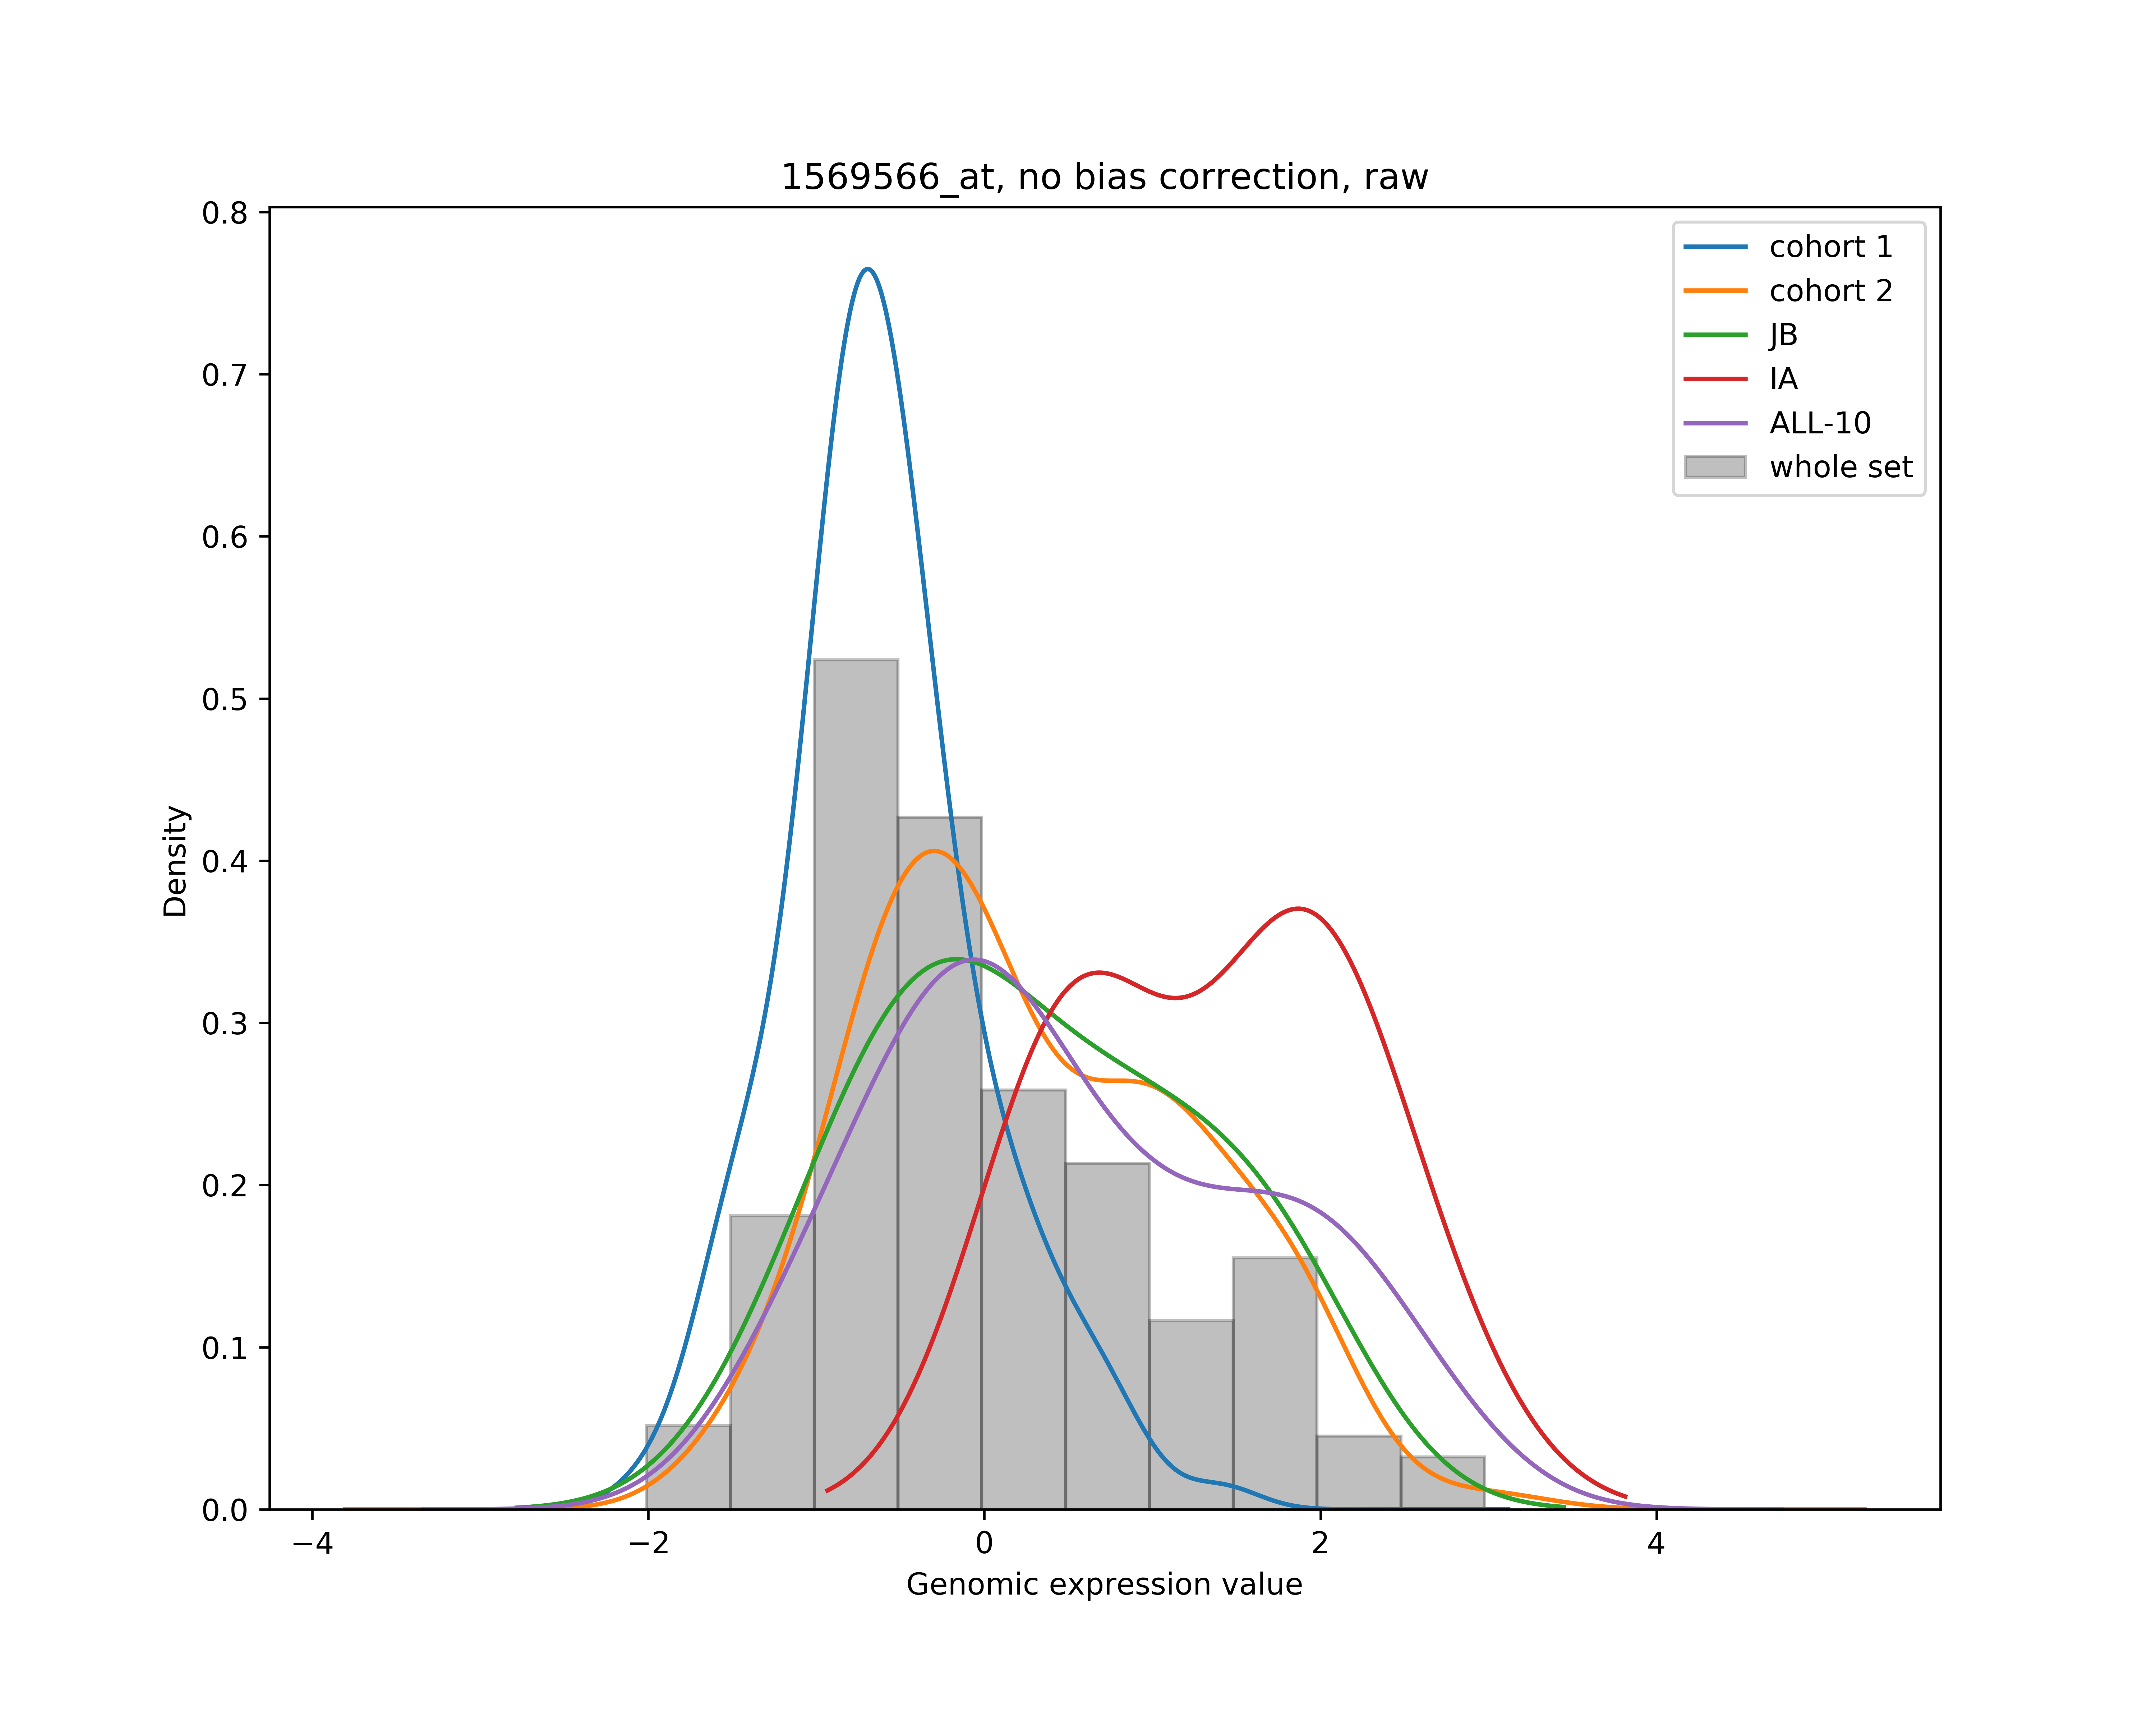
\includegraphics[width=7cm]{images/strong_genome_distribution_noCorrection_noNormalisation}
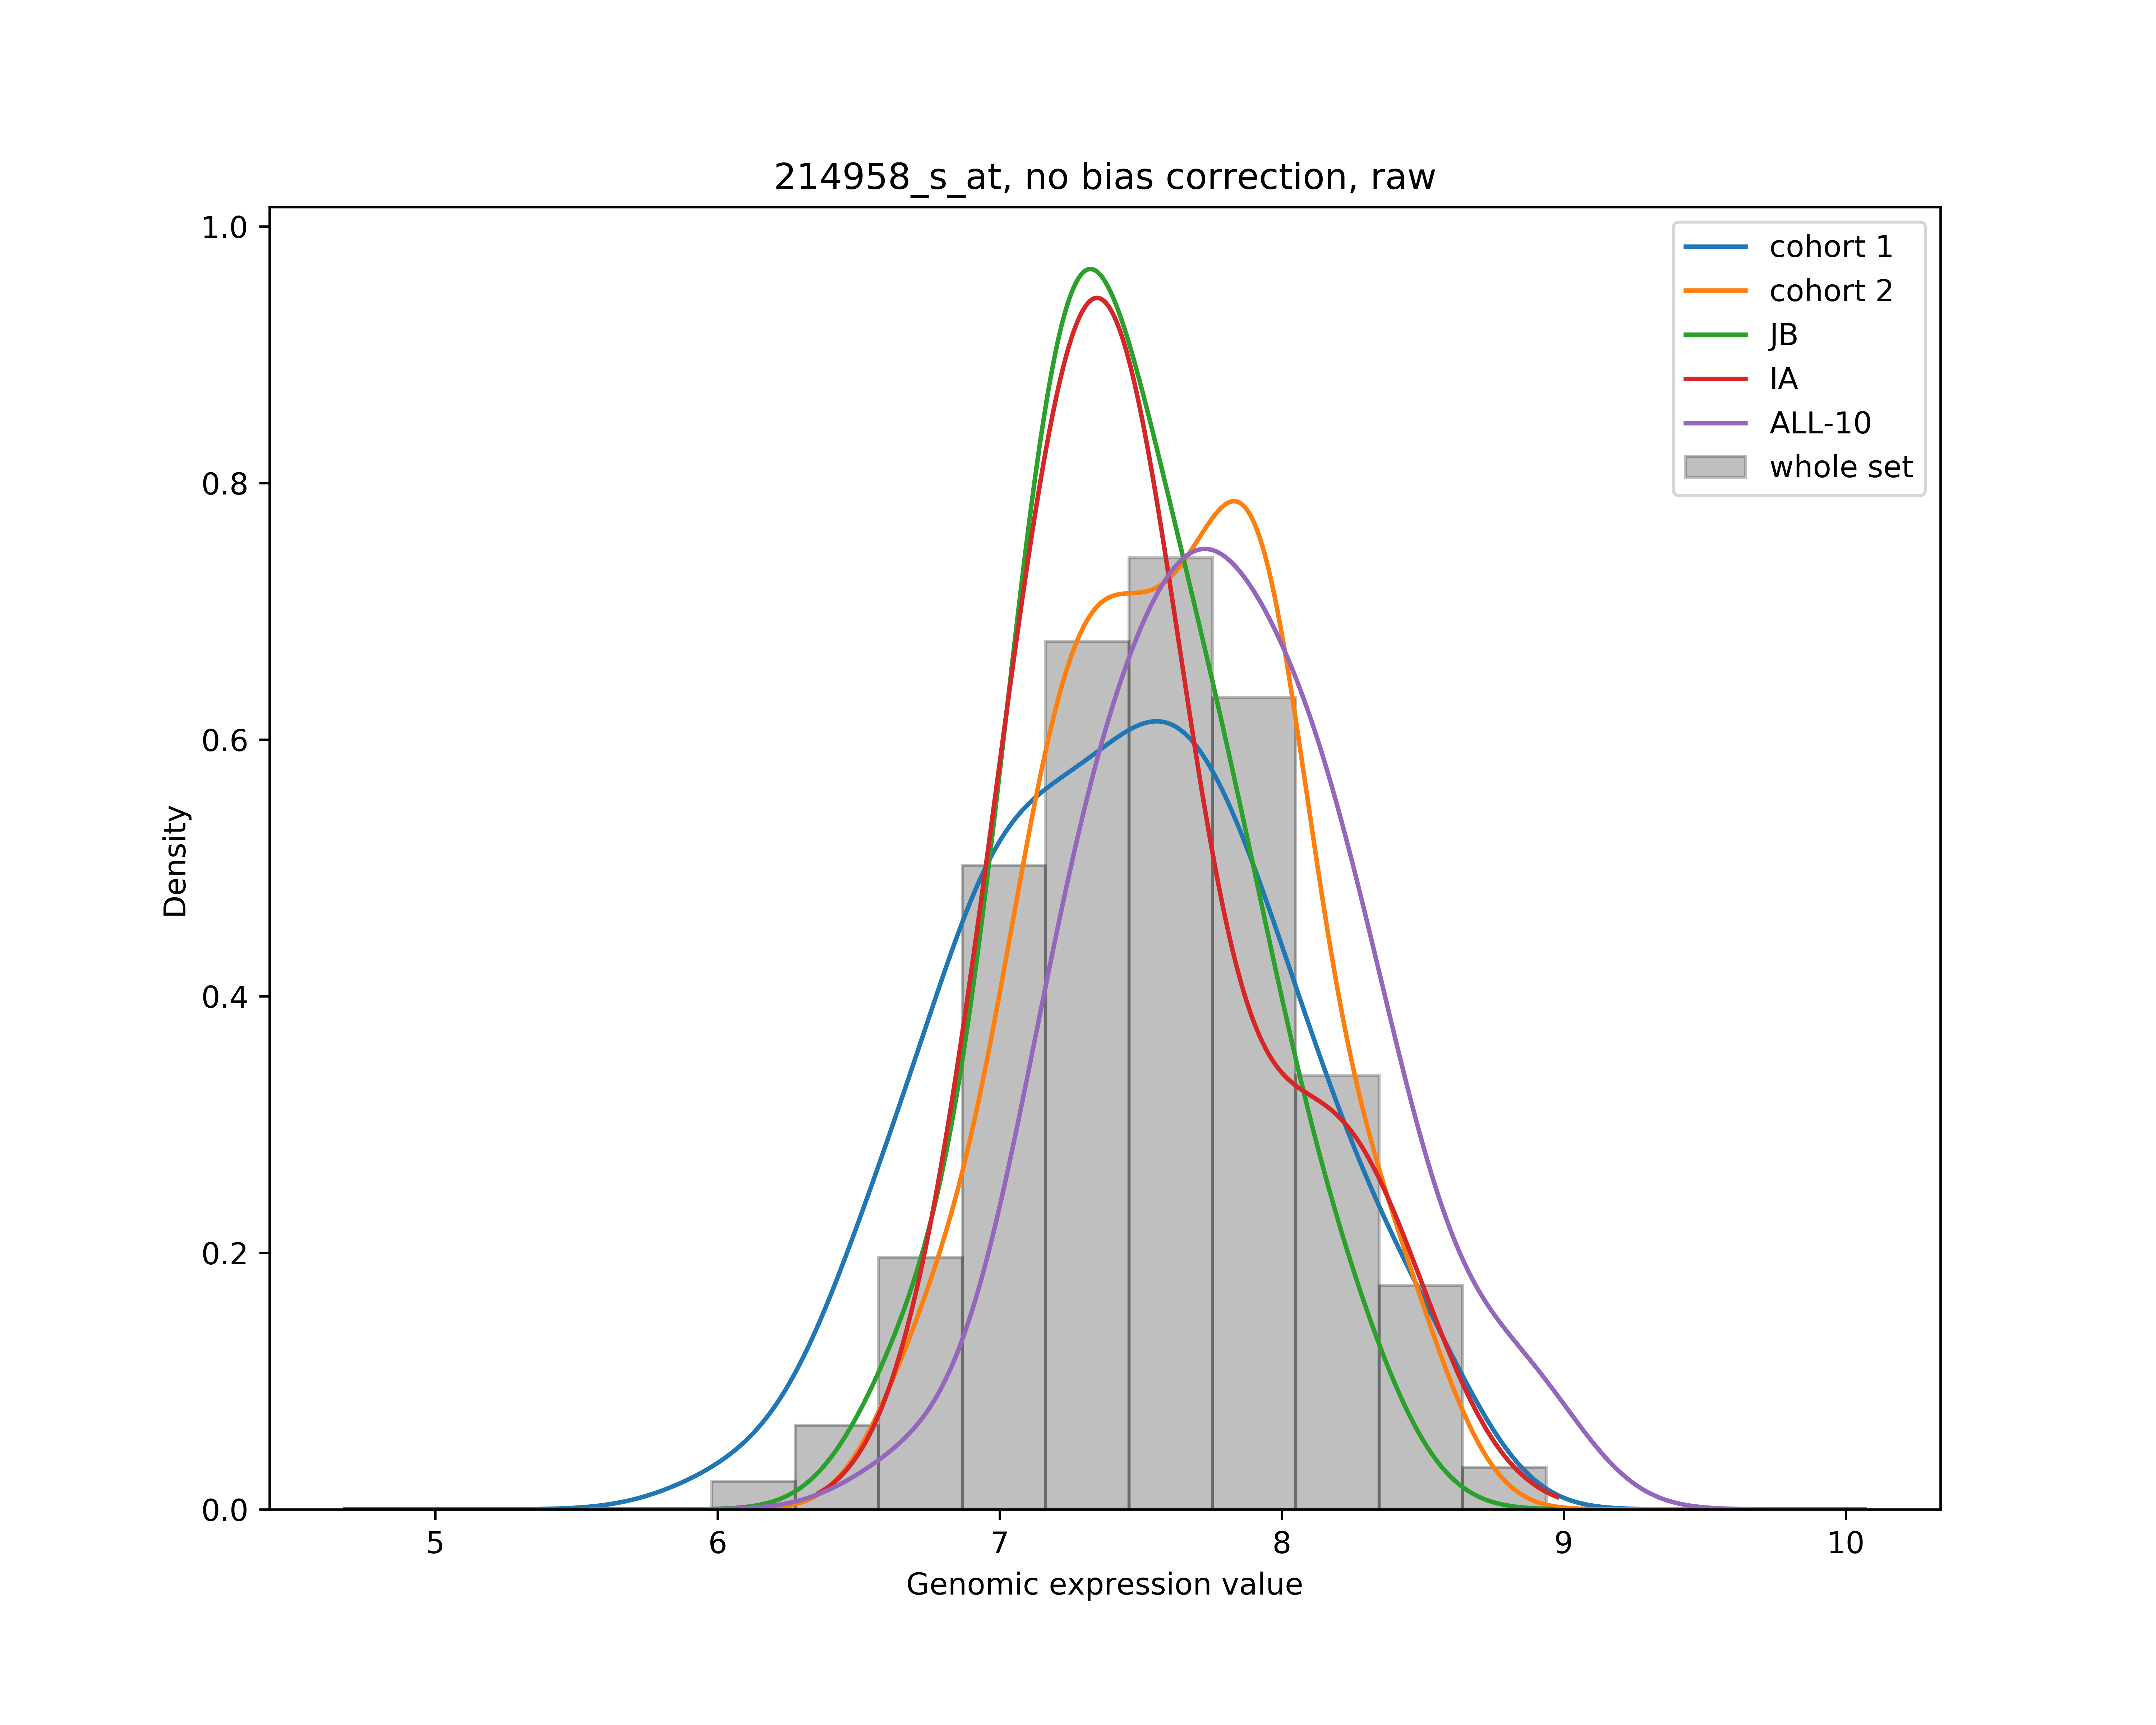
\includegraphics[width=7cm]{images/weak_genome_distribution_noCorrection_noNormalisation}
\caption{Two sets of distributions prior the bias correct, for, (left) a strong predictor and (right) a weak predictor}
\label{fig:expression_distribution_cohorts}
\end{figure}
%
\begin{figure}[htp!]
\centering
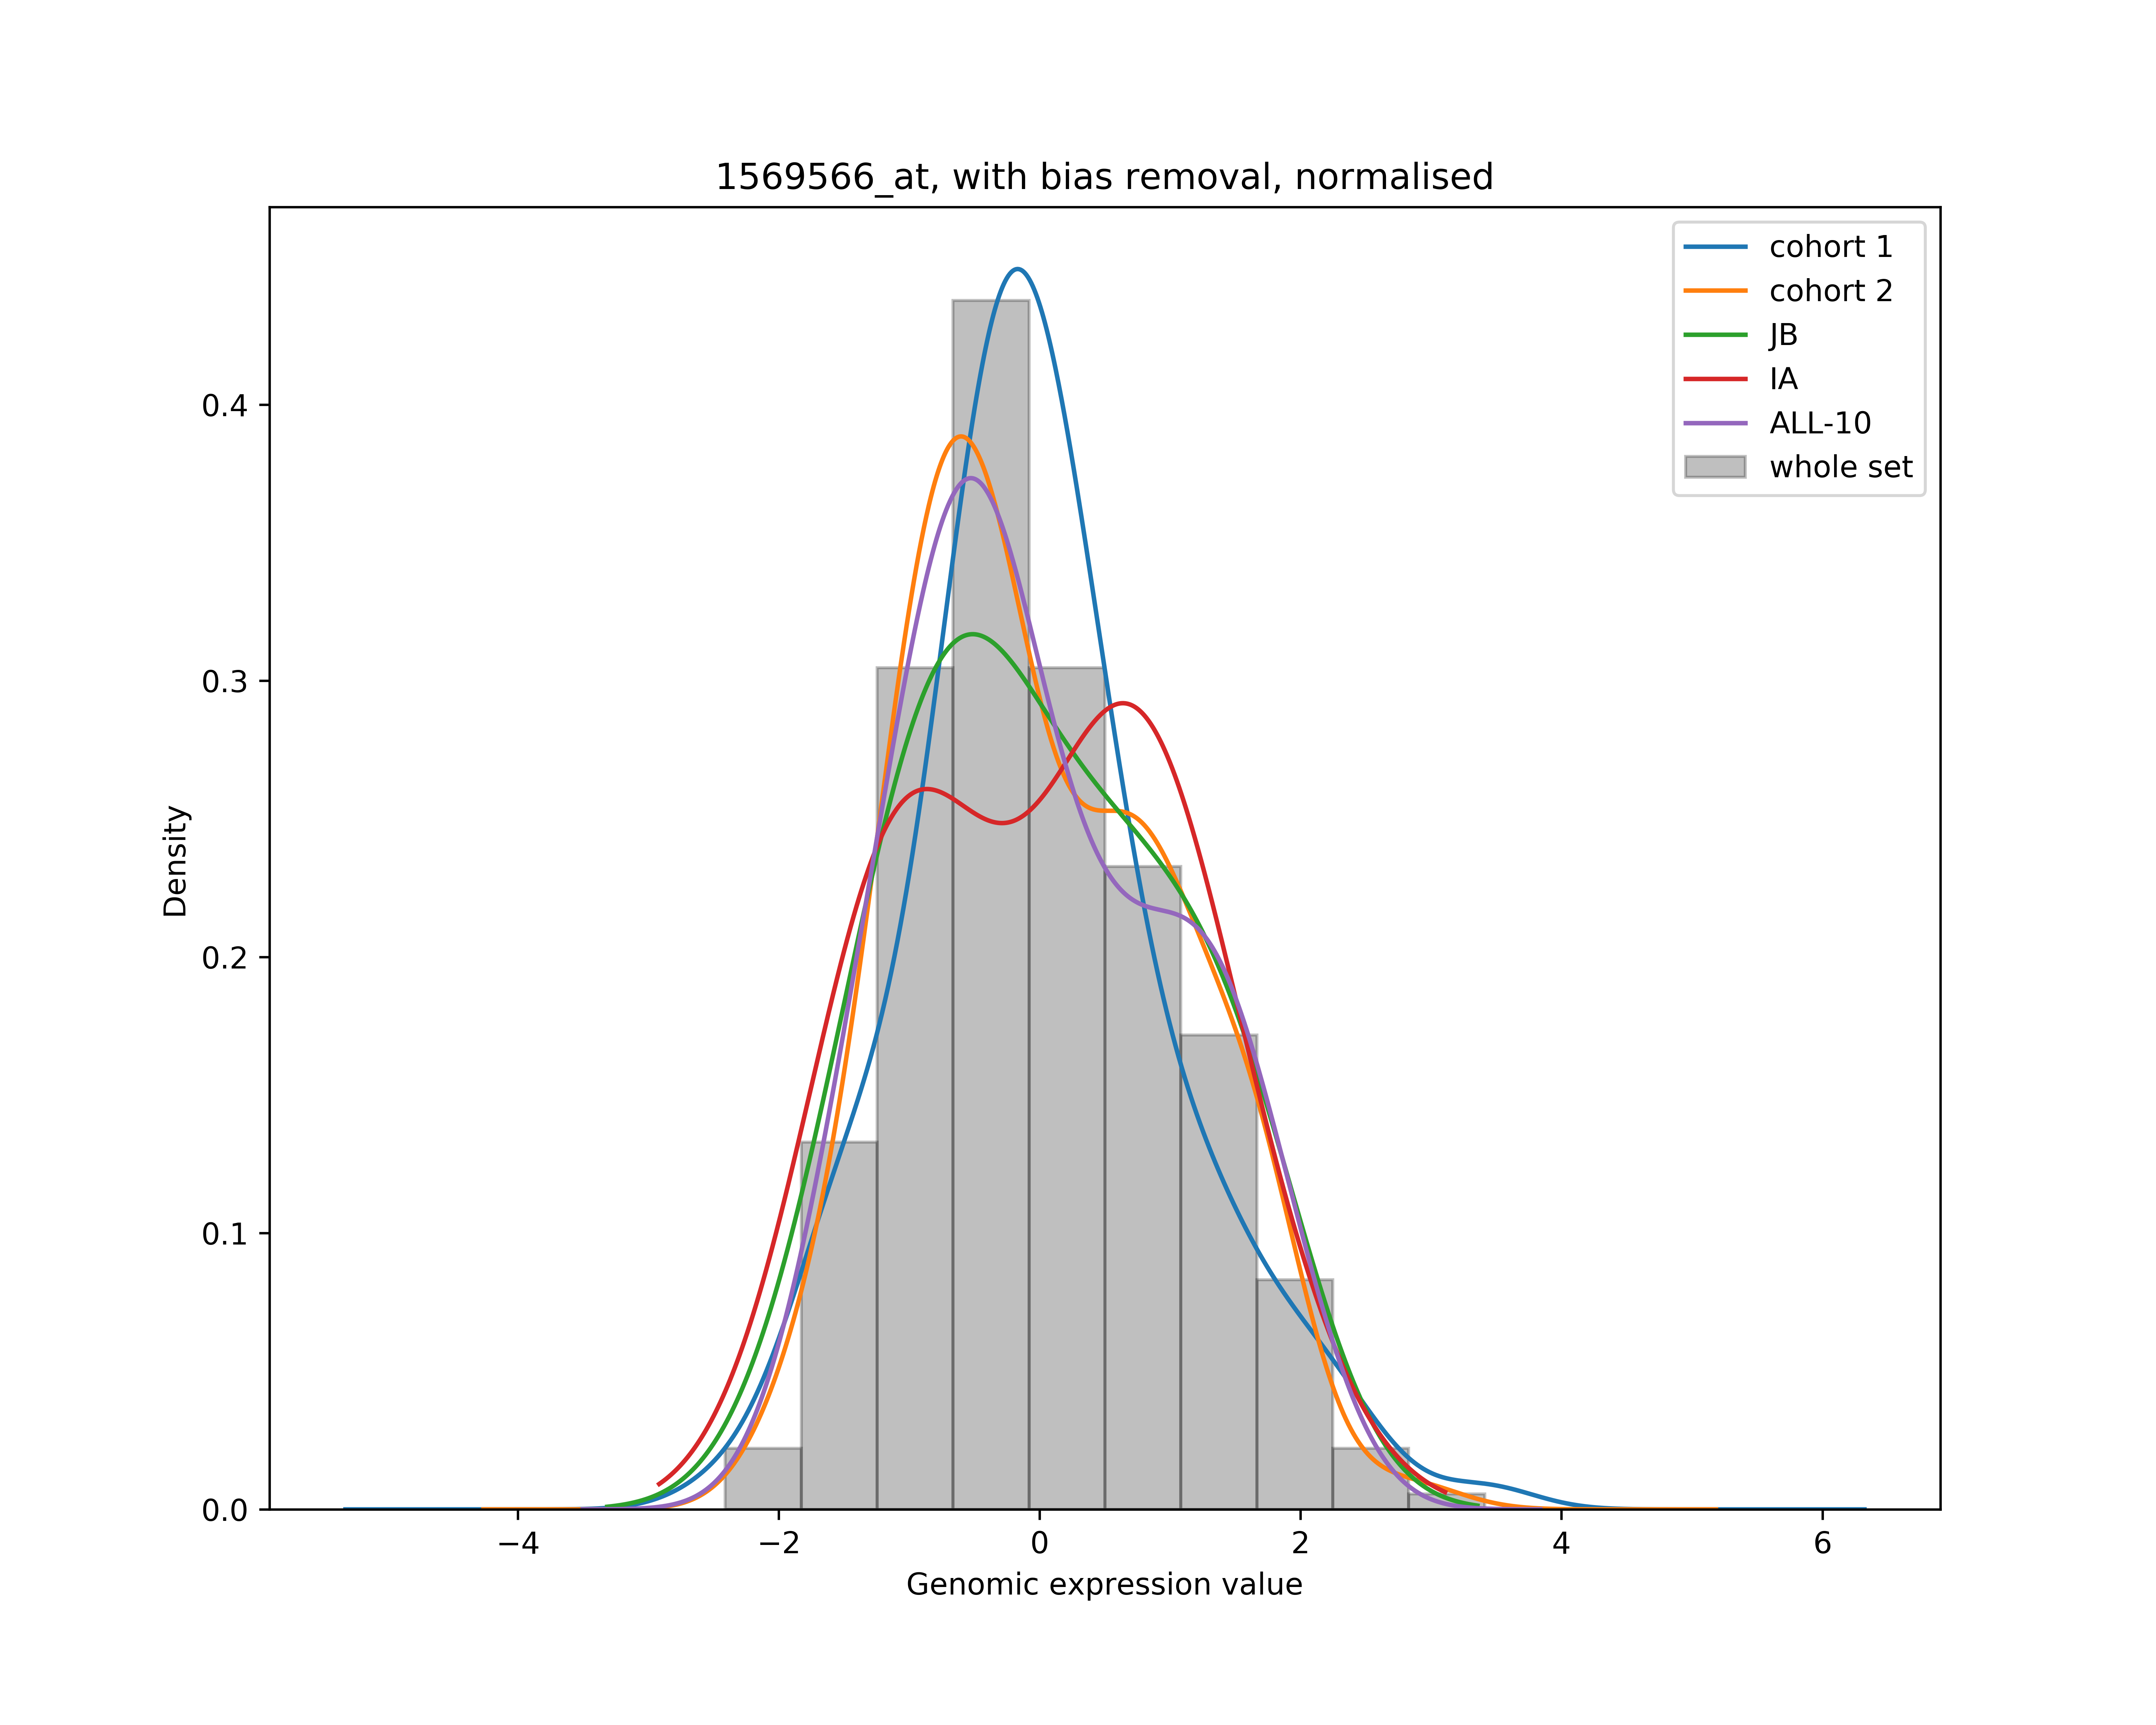
\includegraphics[width=7cm]{images/strong_genome_distribution_withCorrection_standardNormalisation}
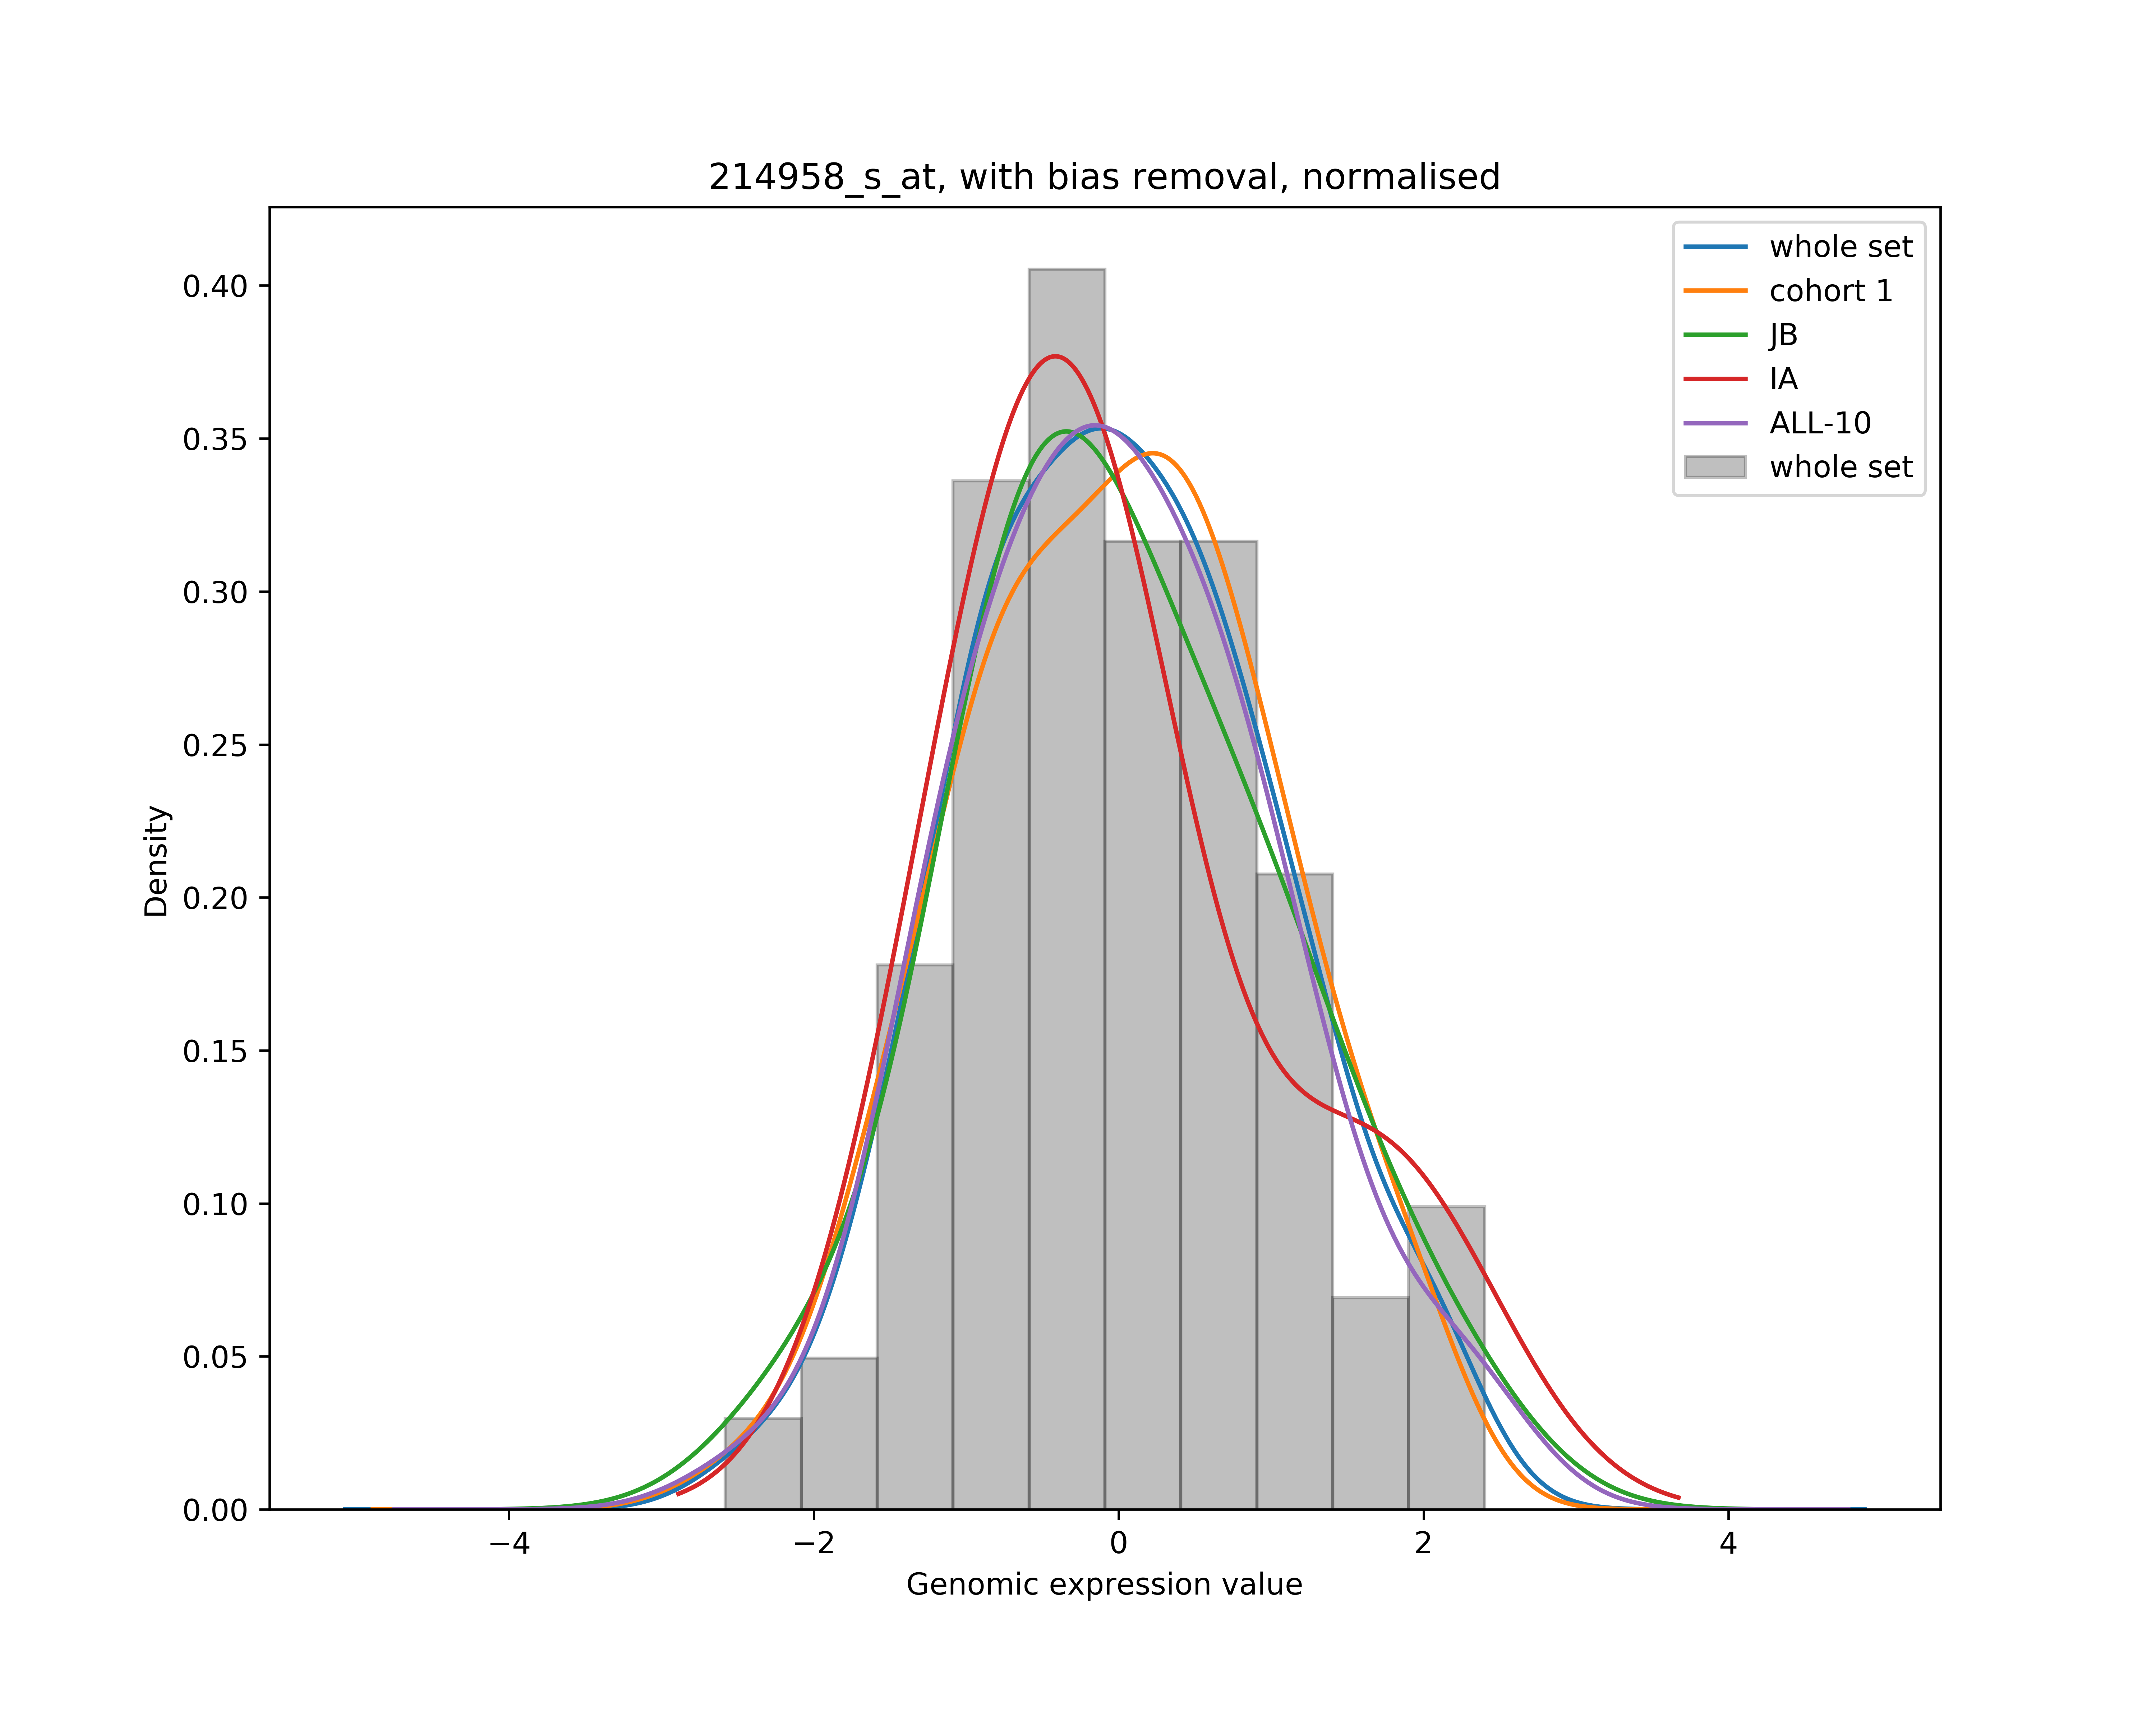
\includegraphics[width=7cm]{images/weak_genome_distribution_withCorrection_standardNormalisation}
\caption{Two sets of distributions with L/S cohort correct, for, (left) a strong predictor and (right) a weak predictor}
\label{fig:expression_distribution_cohorts_withBiasCorrection}
\end{figure}
%Strong: 1569566_at, 223748_at, 223017_at, 1568713_a_at, 201015_s_at
%Weak: 214958_s_at, 200934_at, 207908_at, 205107_s_at, 243806_at
%
There are various more elaborate methods to remove bias such as the SVD-based method from Alter et al.\cite{Alter2000}, the 
PCA-based bias removal methods EIGENSTRAT by Price et al.\cite{Price2006}, MANCIE by Zang et al.\cite{Zang2016}, the distance weighted discrimination (DWD)
approach from Benito et al.\cite{Benito2005} or the ComBat method by Johnson et al.\cite{Johnson2007} who apply an empirical Bayes approach. 
A comparison of bias removal methods is out of scope for this work, for more details we refer the reader to Johnson et al\cite{Johnson2007}.
The basic underlying assumption for all methods is that the samples are stratified over the cohorts, i.e. that in terms
of patients each cohort represents a random selection from the total set of patients. Also, it is assumed that 
the distribution has only one mode. In figures \ref{fig:expression_distribution_cohorts} and \ref{fig:expression_distribution_cohorts_withBiasCorrection}
we show examples of distributions for two different genomes without and with bias removal respectively.

\subsection{Dimension reduction}
%
We considered several dimension reduction techniques such as Principal Component Analysis (PCA, see e.g. Shlens\cite{Shlens2014}), 
Linear Discriminant Analysis (LDA) and the False discovery rate (FDR, see Yoav and Hochberg\cite{Yoav1995}). \\ 
%
PCA is basically a transformation of the feature space based on the eigenvectors 
of the covariance matrix and can be applied to the entire dataset, including the test set.
Using the eigenvectors of the covariance matrix as the basis for the features ensures maximal
variance perpendicular to the coordinate axes. This is a coarse of saying that we maximize the information
content per dimension. The downside is that we obfuscate the biological meaning of the features: any value in the feature set of the transformed matrix is now a linear combination 
of $N$ genome expression values, where $N$ is the number of dimensions. \\
%
In LDA we try to find a linear transformation that maximizes the seperation 
\textbf{between} classes with respect to the seperation \textbf{within} classes, requiring two
covariance matrices. LDA requires availability of the classification label for fitting, hence the transformation is biased to the training set, 
also the features are obfuscated similar to PCA. For both LDA and PCA we need to select the number of dimensions a priori. Furthermore 
we are restricted to a minimum number of dimensions equal to the number of samples. Particularly suited for the dimension reduction
of problems with more dimensions than samples is Partial Least Squares Discriminant Analysis (PLS-DA). (TO-DO literature reference or explanation)  \\ 
%
The FDR method is basically a feature selection based on a minimum statistical seperarability of the distributions over the different classes.
This minimum seperability is in this case the $p$-value for the rejection of the null hypothesis that the samples are drawn from the same distribution, this
$p$-value is usually denoted by $\alpha$.  \\ \\ 
%
Because the Covariance or linear-discrimination based transformation obfuscates the biological meaning of the feature vectors
we choose the FDR method as the most suitable method to reduce the number of dimensions. Also, the FDR method is commonly applied in genomic research
(TO-DO add literature). \\
We apply the FDR method with the Benjamin-Hochberg approach and the ANOVA model to compare the distributions with a maximum $p$-value set at $0.05$. \\ % ANOVA versus Wilcoxon, Mann-Whitney U
%
Arguably, a shortcoming of the FDR method is that, as for LDA, it has a bias towards the training set because it dismisses features solely
on the basis of variance across the different classifications which are obviously not available for the test set. Another shortcoming is that it ignores
feature interdependency, i.e. we may accidentally dismiss feature combinations as predictors because we have removed their constitutive parts, see
e.g. Sun et al.\cite{Sun1996}. \\ 
%
For this reason, the use of a generic dimension reduction technique such as PCA or Autoencoding is advised to improve
the robustness of the model in terms of classification accuracy for larger datasets. For smallers data sets with the number of samples smaller
than the number of dimensions we advise PLS-DA. \\ \\
%
Alternatively one can apply any model generator (to a subset of the data) that produces importance values for the features, e.g. Random Forest (RF), linear Support
Vector Machines (lSVM), Logistic Regression (LR). 
%%
\section{Classification}
%
We will shortly describe the methods used for the predictions and the determination of genome importances.
We will not go in detail on the selection of the method parameters, we refer the reader to the appendix for the
parameter selection.

\subsection{Tree based}

Single decision trees are known to be sensitive to changes in the input data. These ensemble methods 
help to decrease the variance without increasing the bias, i.e. increasing the ability to be generalised. For small
data sets however they are sensitive to overfitting. 
We employ several tree-ensemble methods: Random Forest (RF) by Breiman\cite{Breiman2001}, ExtraTrees (ET) by Geurts et al.\cite{Geurts2006} 
XGBoost (XGB) by Chen and Guestrin\cite{Chen2016} and (Light)GBM (LGBM) by Ke et al.\cite{Ke2017}.
The RF and ET methods are ensemble methods that combine an arbitrary number of decision trees, using bootstrapped samples,
random feature selection and a majority vote classification. The XGB and LGBM methods are ensemble methods 
that apply a technique called gradient boosting by Breiman\cite{Breiman1997}.
%
\subsection{Neural networks}
%
We use two types of neural networks, a Deep Neural Network (DNN) \cite{lecun2015deep} and a Convolutional Neural Network (CNN) \cite{Lecun98}. The main advantage of neural networks is that they can learn non-linear relationships between features. Despite the small sample size, it is interesting to apply neural networks in this context due to the high dimensionality of the data. Neural networks with multiple layers are proficient in discerning more subtle patterns in the data compared to other approaches. Shallow neural networks have been succesfully applied to similar sets of genetic expression data in the past, such as in \cite{khan2001classification}.
A DNN, as shown in figure \ref{fig:dnn_architecture}, uses several fully connected layers of nodes as a network architecture. A high level explanation of the difference between DNNs and CNNs is that a DNN looks at the entire dataset in each node (layers are fully connected).
While a CNN contains operations that allow it to focus on smaller subsets of the data (convolutional layers) 
and operations that allow it to filter out irrelevant data (pooling layers). An example of a CNN architecture for image classification is shown in figure \ref{fig:cnn_architecture}.

\begin{figure}[htp]
  \centering{}
  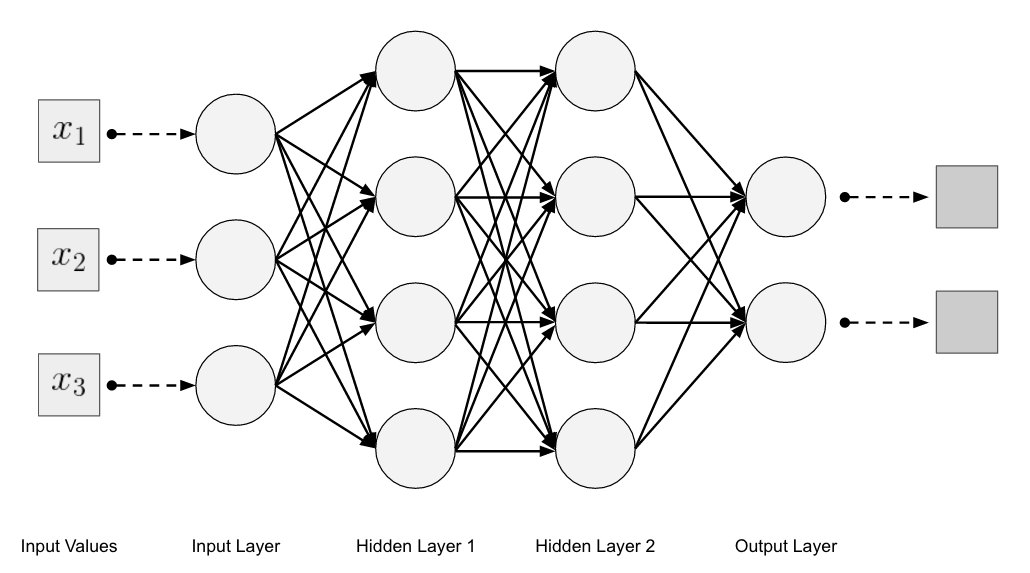
\includegraphics[width=8cm]{images/DNN}
  \caption{A generic architecture for a deep feedforward neural network.}
  \label{fig:dnn_architecture}
\end{figure}

\begin{figure}[htp]
  \centering
  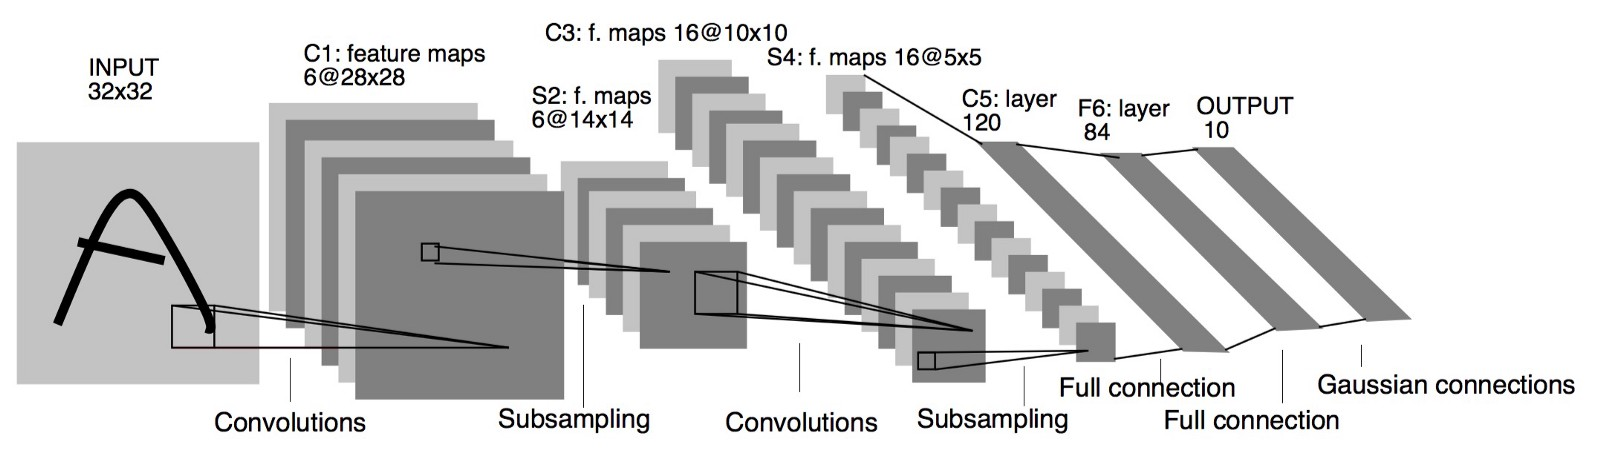
\includegraphics[width=8cm]{images/CNN}
  \caption{A typical convolutional neural network architecture for image classification from \cite{Lecun98}.}
  \label{fig:cnn_architecture}
\end{figure}

Using Local Interpretable Model-Agnostic Explanations (LIME) developed by Ribeiro et al.\cite{Ribeiro2016} 
we can get an idea of the so-called local decision boundary (in feature space) for individual samples which may assist in
understanding the model decision in that particular case. However it is not tractable to discern which features are important
for the final overall model.
%
\subsection{Linear methods}
%
TO-DO: FINISH 
Logistic Regression (LR),..bladiebladie 
Supposedly LR requires about $10$ data points per feature to give stable predictions, the so-called \textit{rule-of-ten}, and it assumes that
the features are independent. \\ 
%
linear Support Vector Machines (lSVM), ..bladiebladie
linear discriminant analysis (LDA),..bladiebladie
%
%Simplicity, transparancy, robustness. However, what we gain in expressiveness we may lose in accuracy.

\subsection{Bayesian methods}
%
Naive Bayes (NB) classification revolves around the chaining of conditional probabilities under the naive assumption
that features are conditionally independent. Naive Bayes has been applied in genomic classification, see e.g. Sandberg et al.\cite{Sandberg2001}, Ferrari and Aitken\cite{Ferrari2006}, DePristo et al.\cite{DePristo2011}. The method is naive because it assumes that the features are independent in determining the probability of a classification. Also, the model is 
zeroeth order dependent on the prior probability of the class, hence, it assumes this prior probability also when applied
outside the training data. As the genomic expression values are continuous we have to apply Gaussian NB specifically; 
with Gaussian NB we assign a Gaussian distribution to each feature per classification. \\ \\
%
Gaussian Processes Classification (GPC) uses Gaussian Processes to model the prior probabilities and tries to find
the conditional class probabilities comparable to Naive Bayes, see e.g. Chu et al.\cite{Chu2005} who applied it to genome sequences. 
The GPC method requires a sampling method such as Markov-Chain-Monte-Carlo which scales quadratically with the dimensionality, hence it is limited to low-dimensional problems. The downside of Bayesian methods, the dependency on prior probabilities (i.e. bias), is also their strength, as the model is much less prone to overfitting. 
%
\subsection{Stacking}
%
For the final predictions we stack the models, combining the predictions of the individual 
models in one final prediction. To do this we use the uncertainty estimation from the model per sample plus the overall accuracy from cross-validation
as weights
\begin{equation*}
 y_i =  \frac{\sum_i 2(\vert \hat{y} - 1/2\vert\beta \hat{y})_i}{\sum_i{2(\vert \hat{y} - 1/2\vert\beta)_i}} 
\end{equation*}
%
\section{Results}
% 
\subsection{Model Evaluation}
%
Model evaluation for training strategy $\mathcal{I}$ is done using the standard $k$-fold cross-validation approach. The data is split into $k$ random folds. In each iteration, a model is trained on $k-1$ folds and tested on the remaining fold. After this procedure we obtain predictions for every sample from a model that is trained on a different part of the data. This gives us a clear idea about how stable the model is and how well it will perform on new data.
%
\subsection{Training strategy $\mathcal{I}$}
%
\begin{table}[htp]
\centering
\begin{tabular}{rlllll}

\textit{method}						& DNN, CNN 		& RF,ET,XGB,LGBM	&  lSVM,LR,LDA		& NB, GPC  			\\
							\hline
RAW, $d=54613$ 						& $71, 71$	 	&  $71, 68, 71, 66$	&  $72, 62, X$		&  $62, 56$  			\\
FDR $\alpha=0.01$, $d\approx 12$ 			& $96, X$  		&  $86, 84, 80, 81$	&  $82, 87, \mathbf{88}$&  $\mathbf{88}, 86$  		\\
FDR $\alpha=0.02$, $d\approx 15$ 			& $95, X$	  	&  $86, 85, 82, 83$	&  $79, 84, 86$		&  $86, 84$			\\
FDR $\alpha=0.03$, $d\approx 57$ 			& $99, \mathbf{92}$  	&  $81, 82, 75, 84$	&  $89, 89, 82$		&  $86, 88$			\\
FDR $\alpha=0.05$, $d\approx 170$ 			& $99, \mathbf{93}$  	&  $79, 78, 75, 79$	&  $87, 87, 83$		&  $82, 81$			\\
FDR $\alpha=0.1$,  $d\approx 412$ 			& $100,\mathbf{93}$	&  $79, 79, 75, 79$	&  $86, 86, 83$		&  $81, 81$			\\
PLS-DA, $d=100$ 					& $99, 81$		&  $79, 66, 83, 75$	&  $100, 100, 100$	&  $\mathbf{86}, 56$		\\
PLS-DA, $d=200$ 					& $99, 82$		&  $74, 60, 82, 75$	&  $100, 100, 100$  	&  $\mathbf{86}, 56$		\\
PLS-DA, $d=400$ 					& $100, 78$		&  $75, 64, 82, 76$	&  $100, 100, 100$  	&  $\mathbf{86}, 56$		
\end{tabular}
\caption{Training strategy $\mathcal{I}$. Mean accuracies in $\%$ over $10$ runs with $5\%$ added random noise per run, with $10$ folds for the cross-validation. $d$ denotes the number of features}
\label{tab:diversitymetrics}
\end{table}
%
The DNN model is likely overfitted, despite the added $5\%$ noise. If we use PLS we see overfitting for lSVM, LDA and LR, again despite the noise.
The model overfitting can be a result of the small number of samples with respect to the number of dimensions. Overall, the accuracy does not increase 
with the number of features. This may be due to the noise generated by non-important genomes leading to a high model variance. The linear methods perform well
which may be due to the low effective dimensionality where a few genomic expressions dominate \textit{and} have a monotonous correlation with the classification probability. \\ \\
% Furthermore it is somewhat remarkable that Gaussian Naive Bayes performs better than Gaussian Processes Classification as the latter should be a more general version of the 
% former, this may be due to sampling-induced errors.
%
To further increase the accuracy of our predictions (without increasing the bias) we can apply a so-called ensemble method that combines the predictors
into one predictor. \\ \\
%
TABLE of prediction accuracies using ensemble methods  \\ % majority vote, unweighted average, weighted by accuracy, weighted by uncertainty 
PLOT of prediction certainty (i.e. proba's)
%
\subsection{Training strategy $\mathcal{II}$}

% Is this correct? Seperate bias removal for each cohort might change the overall ordering of a feature -> which does make a tree sensitive to bias removal
% good point: it could also be that the tree methods mostly ignore the weak features automagically but I will need to verify.
% Tree methods do their own feature selection, if it is not possible to make a decent split of the data with a certain feature itll be ignored, however since the sample size is so small it still might be able to make a decent split on a shit feature, because of pure luck. I was talking about the bias removal tho, which doesn't have much to do with feature selection?
% Well, without bias removal it may be that samples contradict eachother over different cohorts.

\section{Post-processing}
%
\begin{figure}[htp!]
\centering
% met width = 7 cm kunnen we het naast elkaar plotten
\subfloat[]{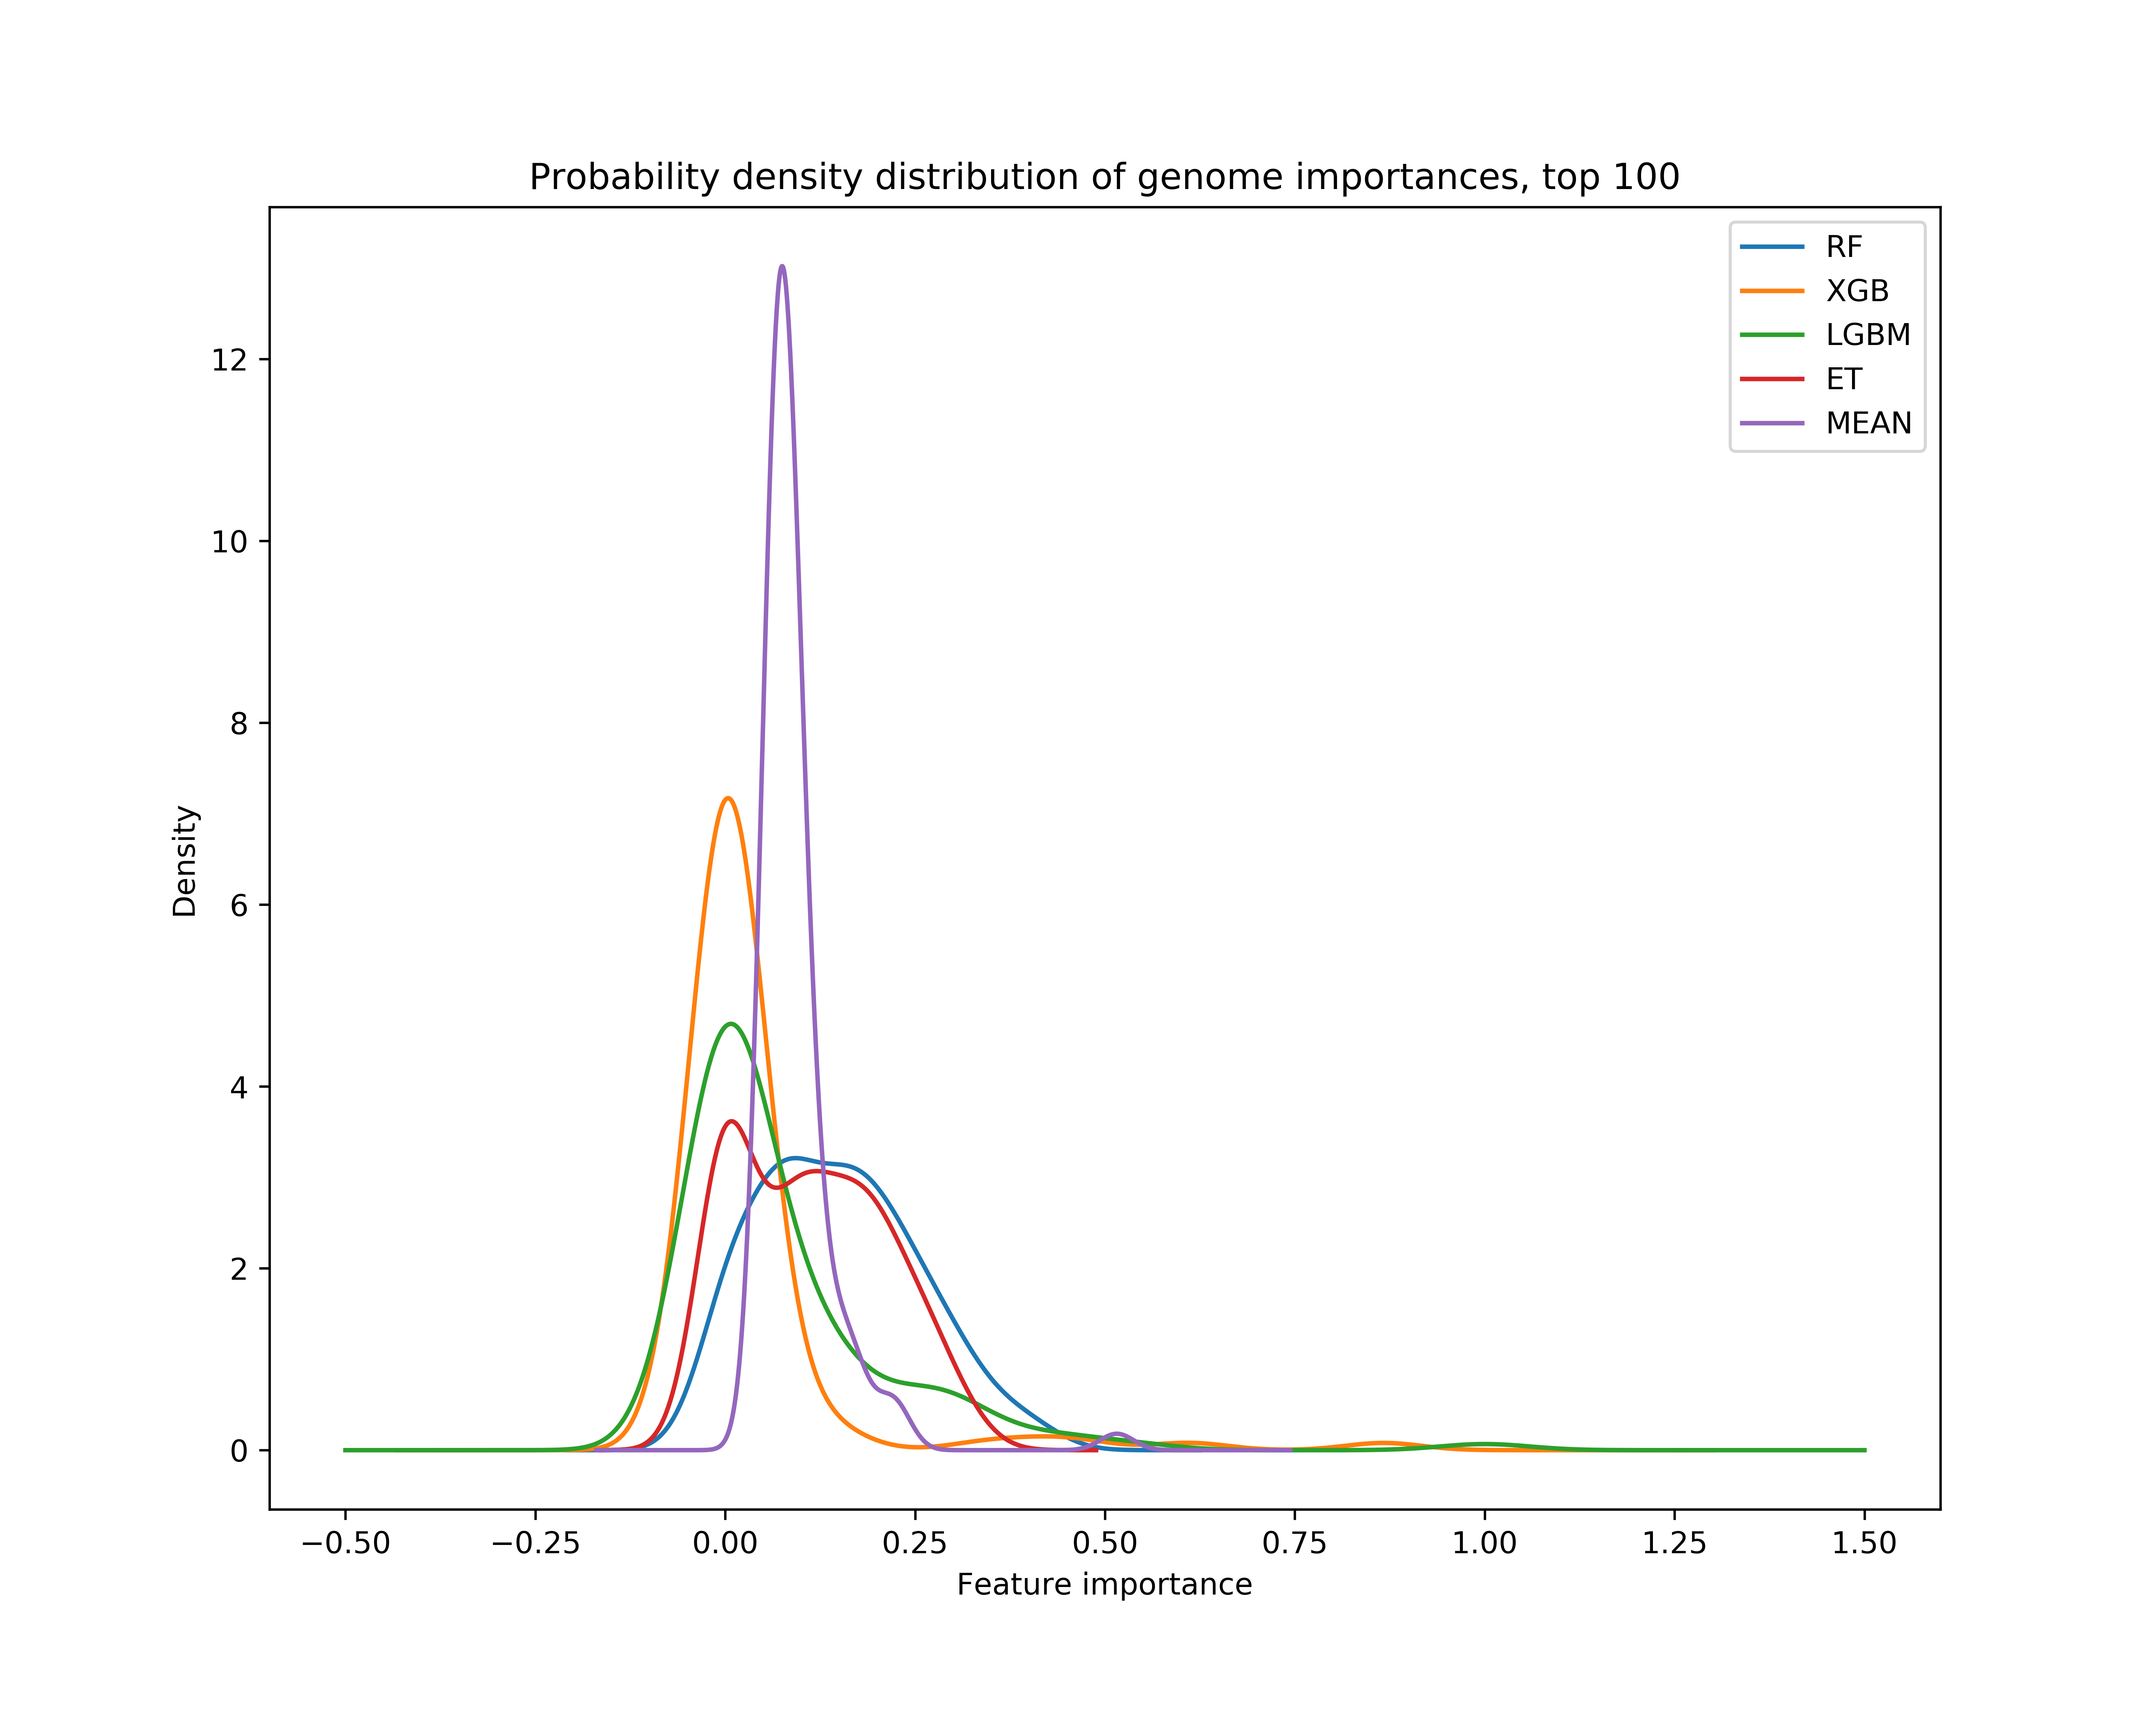
\includegraphics[width=7cm]{images/genome_importances_distribution_top100}}
\vspace{0.5cm}
\subfloat[]{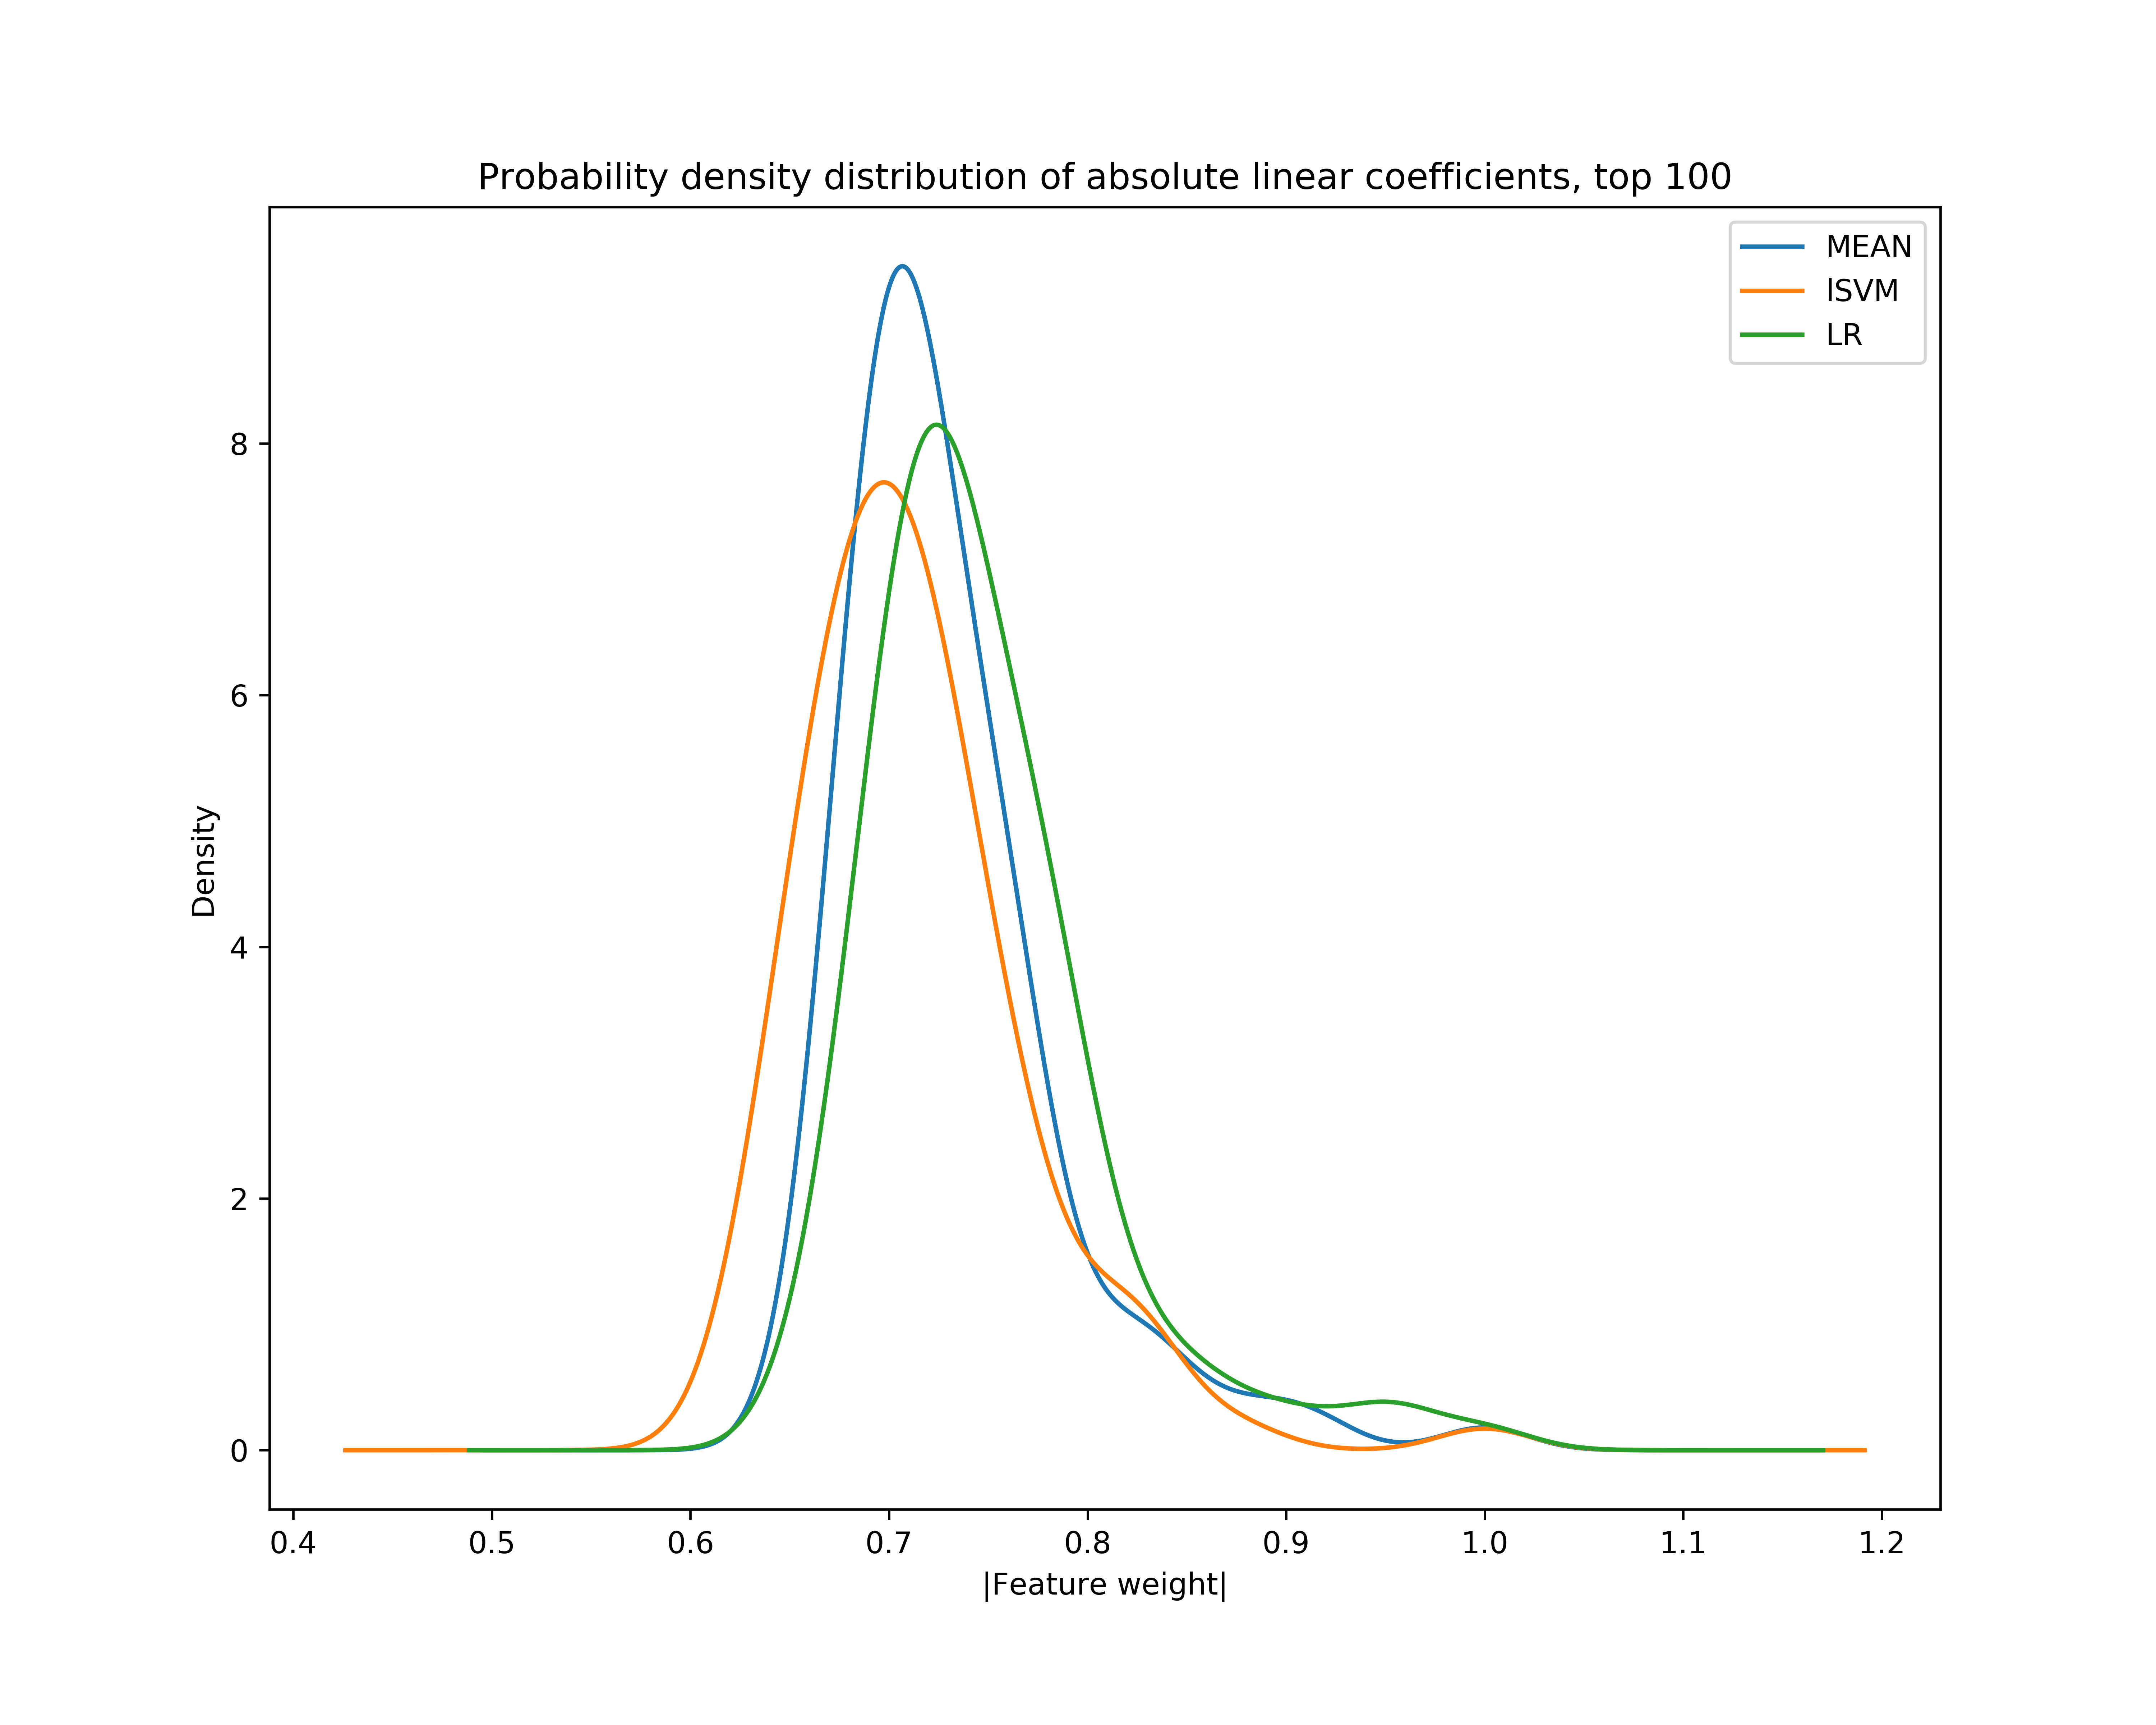
\includegraphics[width=7cm]{images/genome_coeffs_distribution_top100}}
\caption{Distribution of (a) weights and (b) importances associated with genomic expression values with regard to their
influence on several models for training strategy $\mathcal{I}$}
\label{fig:weightsFromModels}
\end{figure}
%
In figure \ref{fig:weightsFromModels} we present the density distributions of the feature weights/importances that
are part of the models generated using all available features (i.e. no feature selection or dimension reduction), 
clearly only few genomic expression values have a significant individual contribution. The distribution of importances that are
produced by the tree methods are dominated by the large number of insignificant features. 
If we apply the FDR method with $\alpha=0.05$ we reduce the dimensionality to about $200$ features. We then train the
models on the reduced data set so we get a smoother distribution of importances, see figure \ref{fig:weightsFromModels}, 
and the same for the weights obtained from the lSVM and LR methods, see figure \ref{fig:coeffsFromModels}.
%
\begin{figure}[htp!]
\centering
% met width = 7 cm kunnen we het naast elkaar plotten
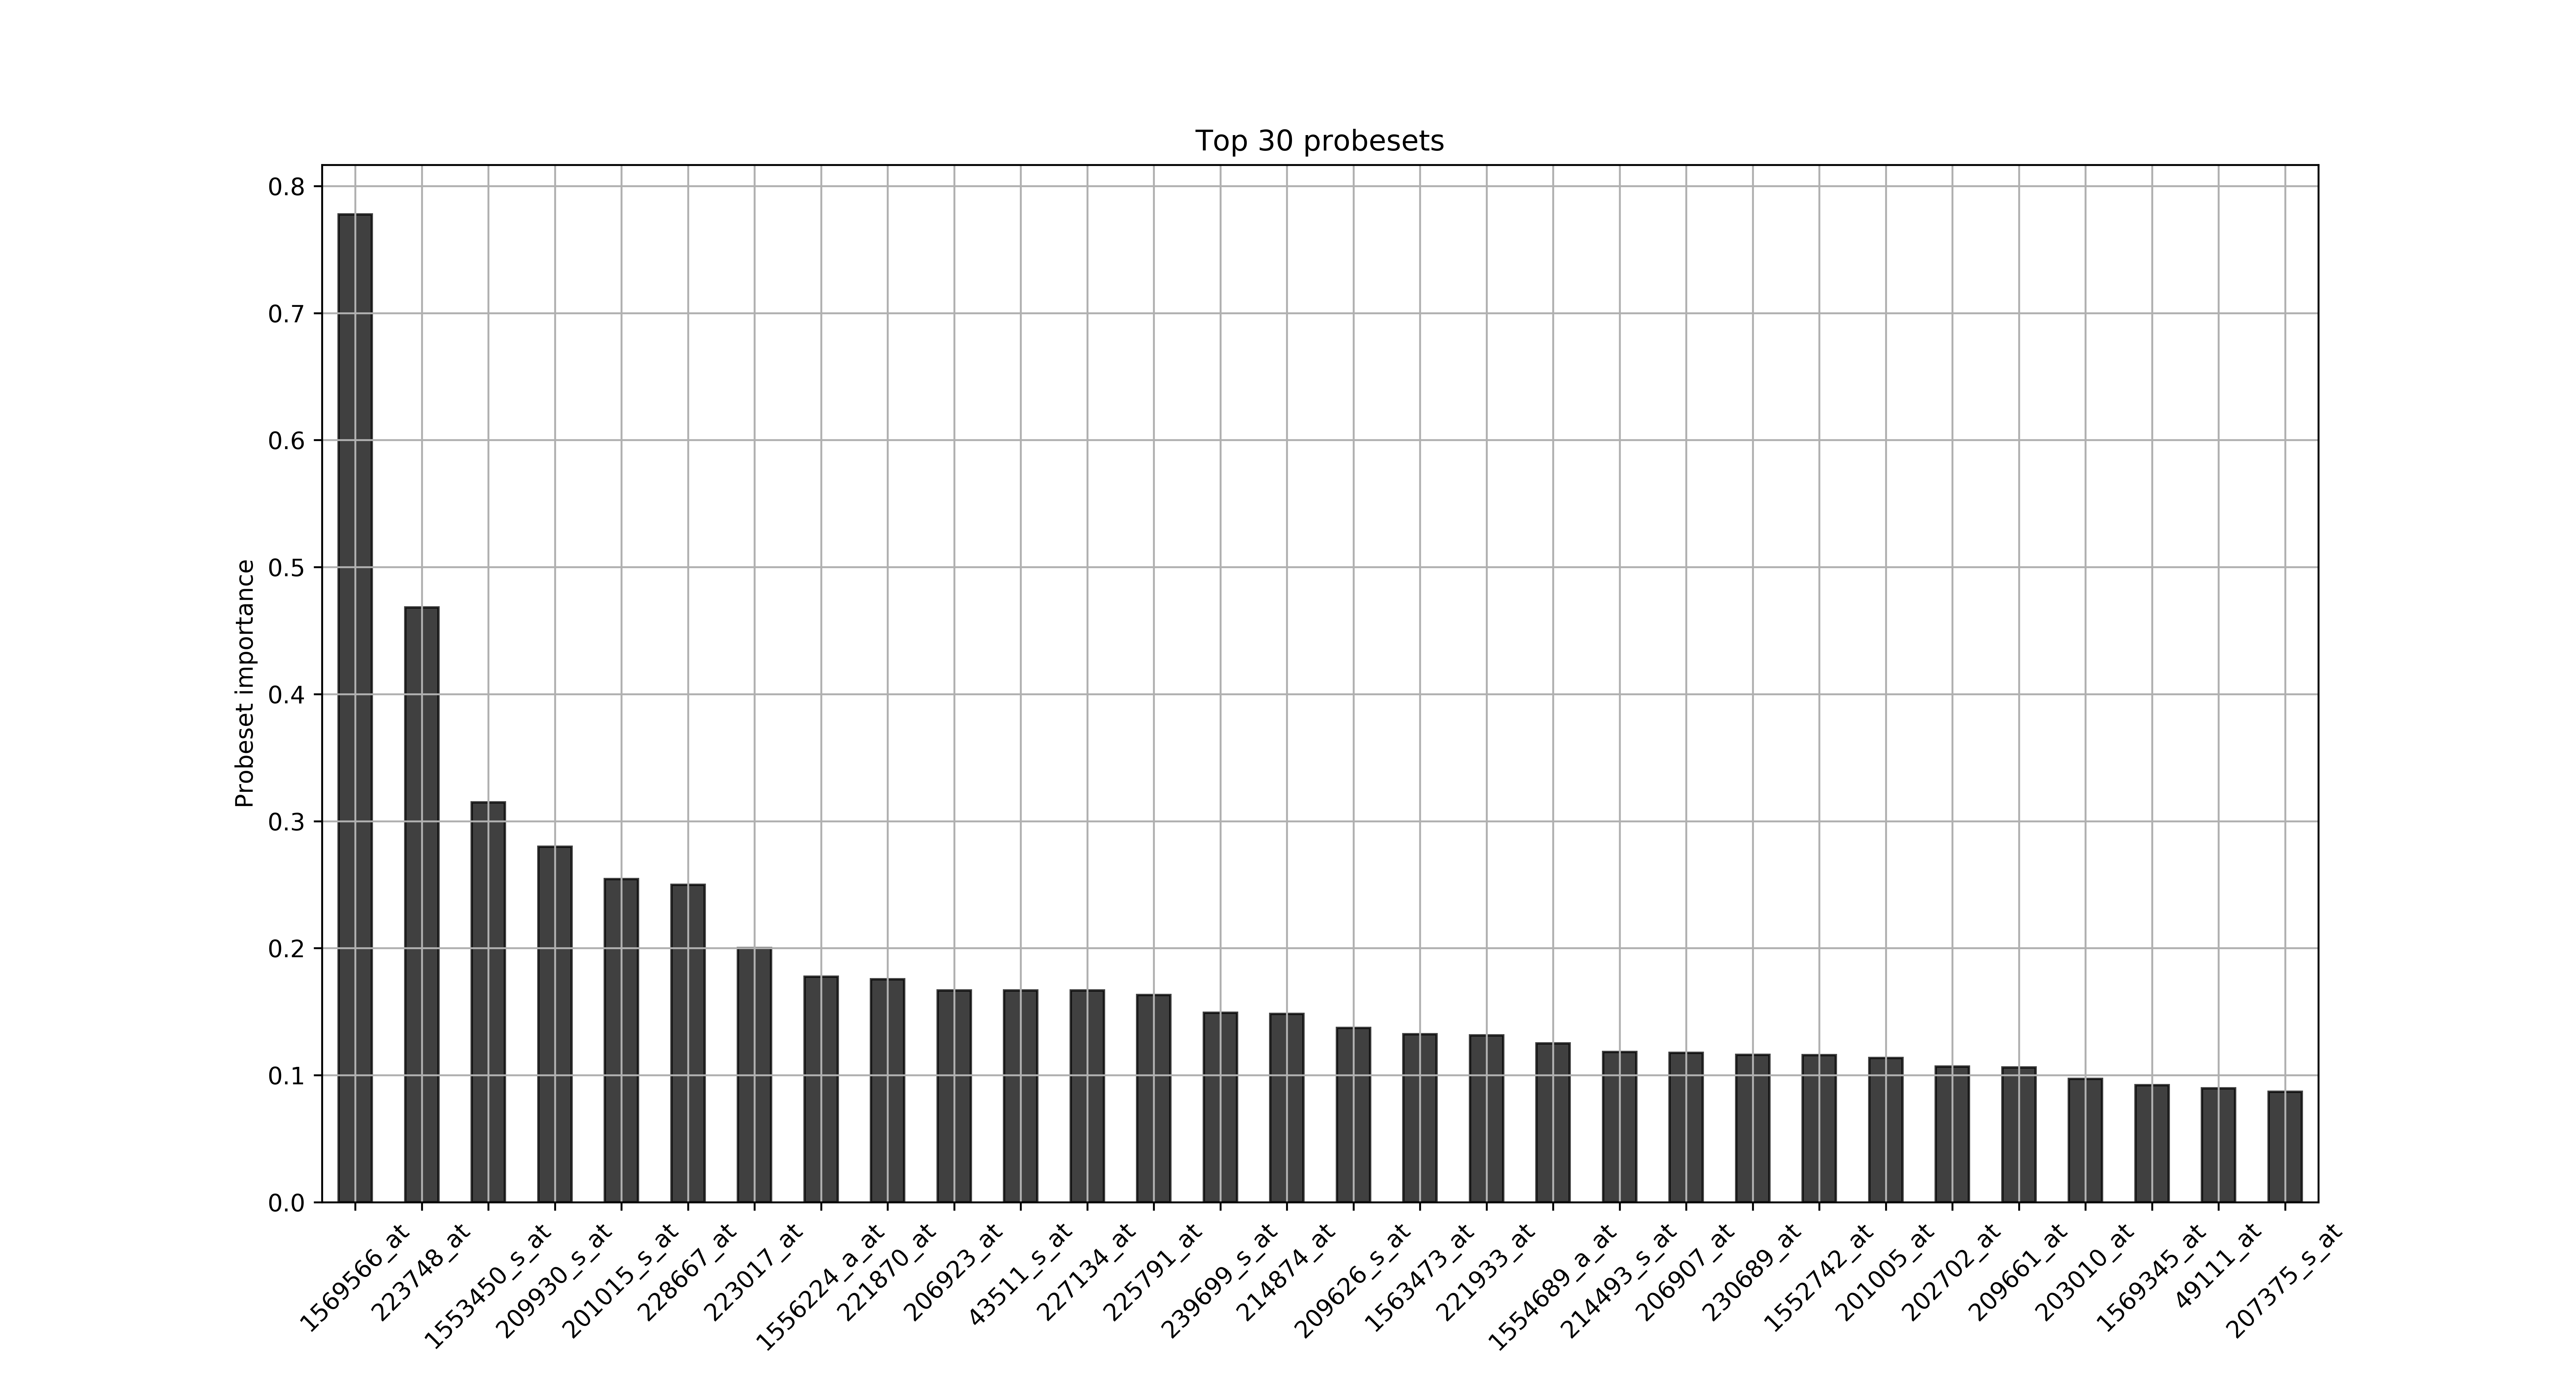
\includegraphics[width=12cm]{images/top30_importances_FDR005}
\caption{Top $30$ probesets in terms of median absolute importances (weights) for the RF, ET, XGB and LGBM models}
\label{fig:weightsFromModels}
\end{figure}
%
\begin{figure}[htp!]
\centering
% met width = 7 cm kunnen we het naast elkaar plotten
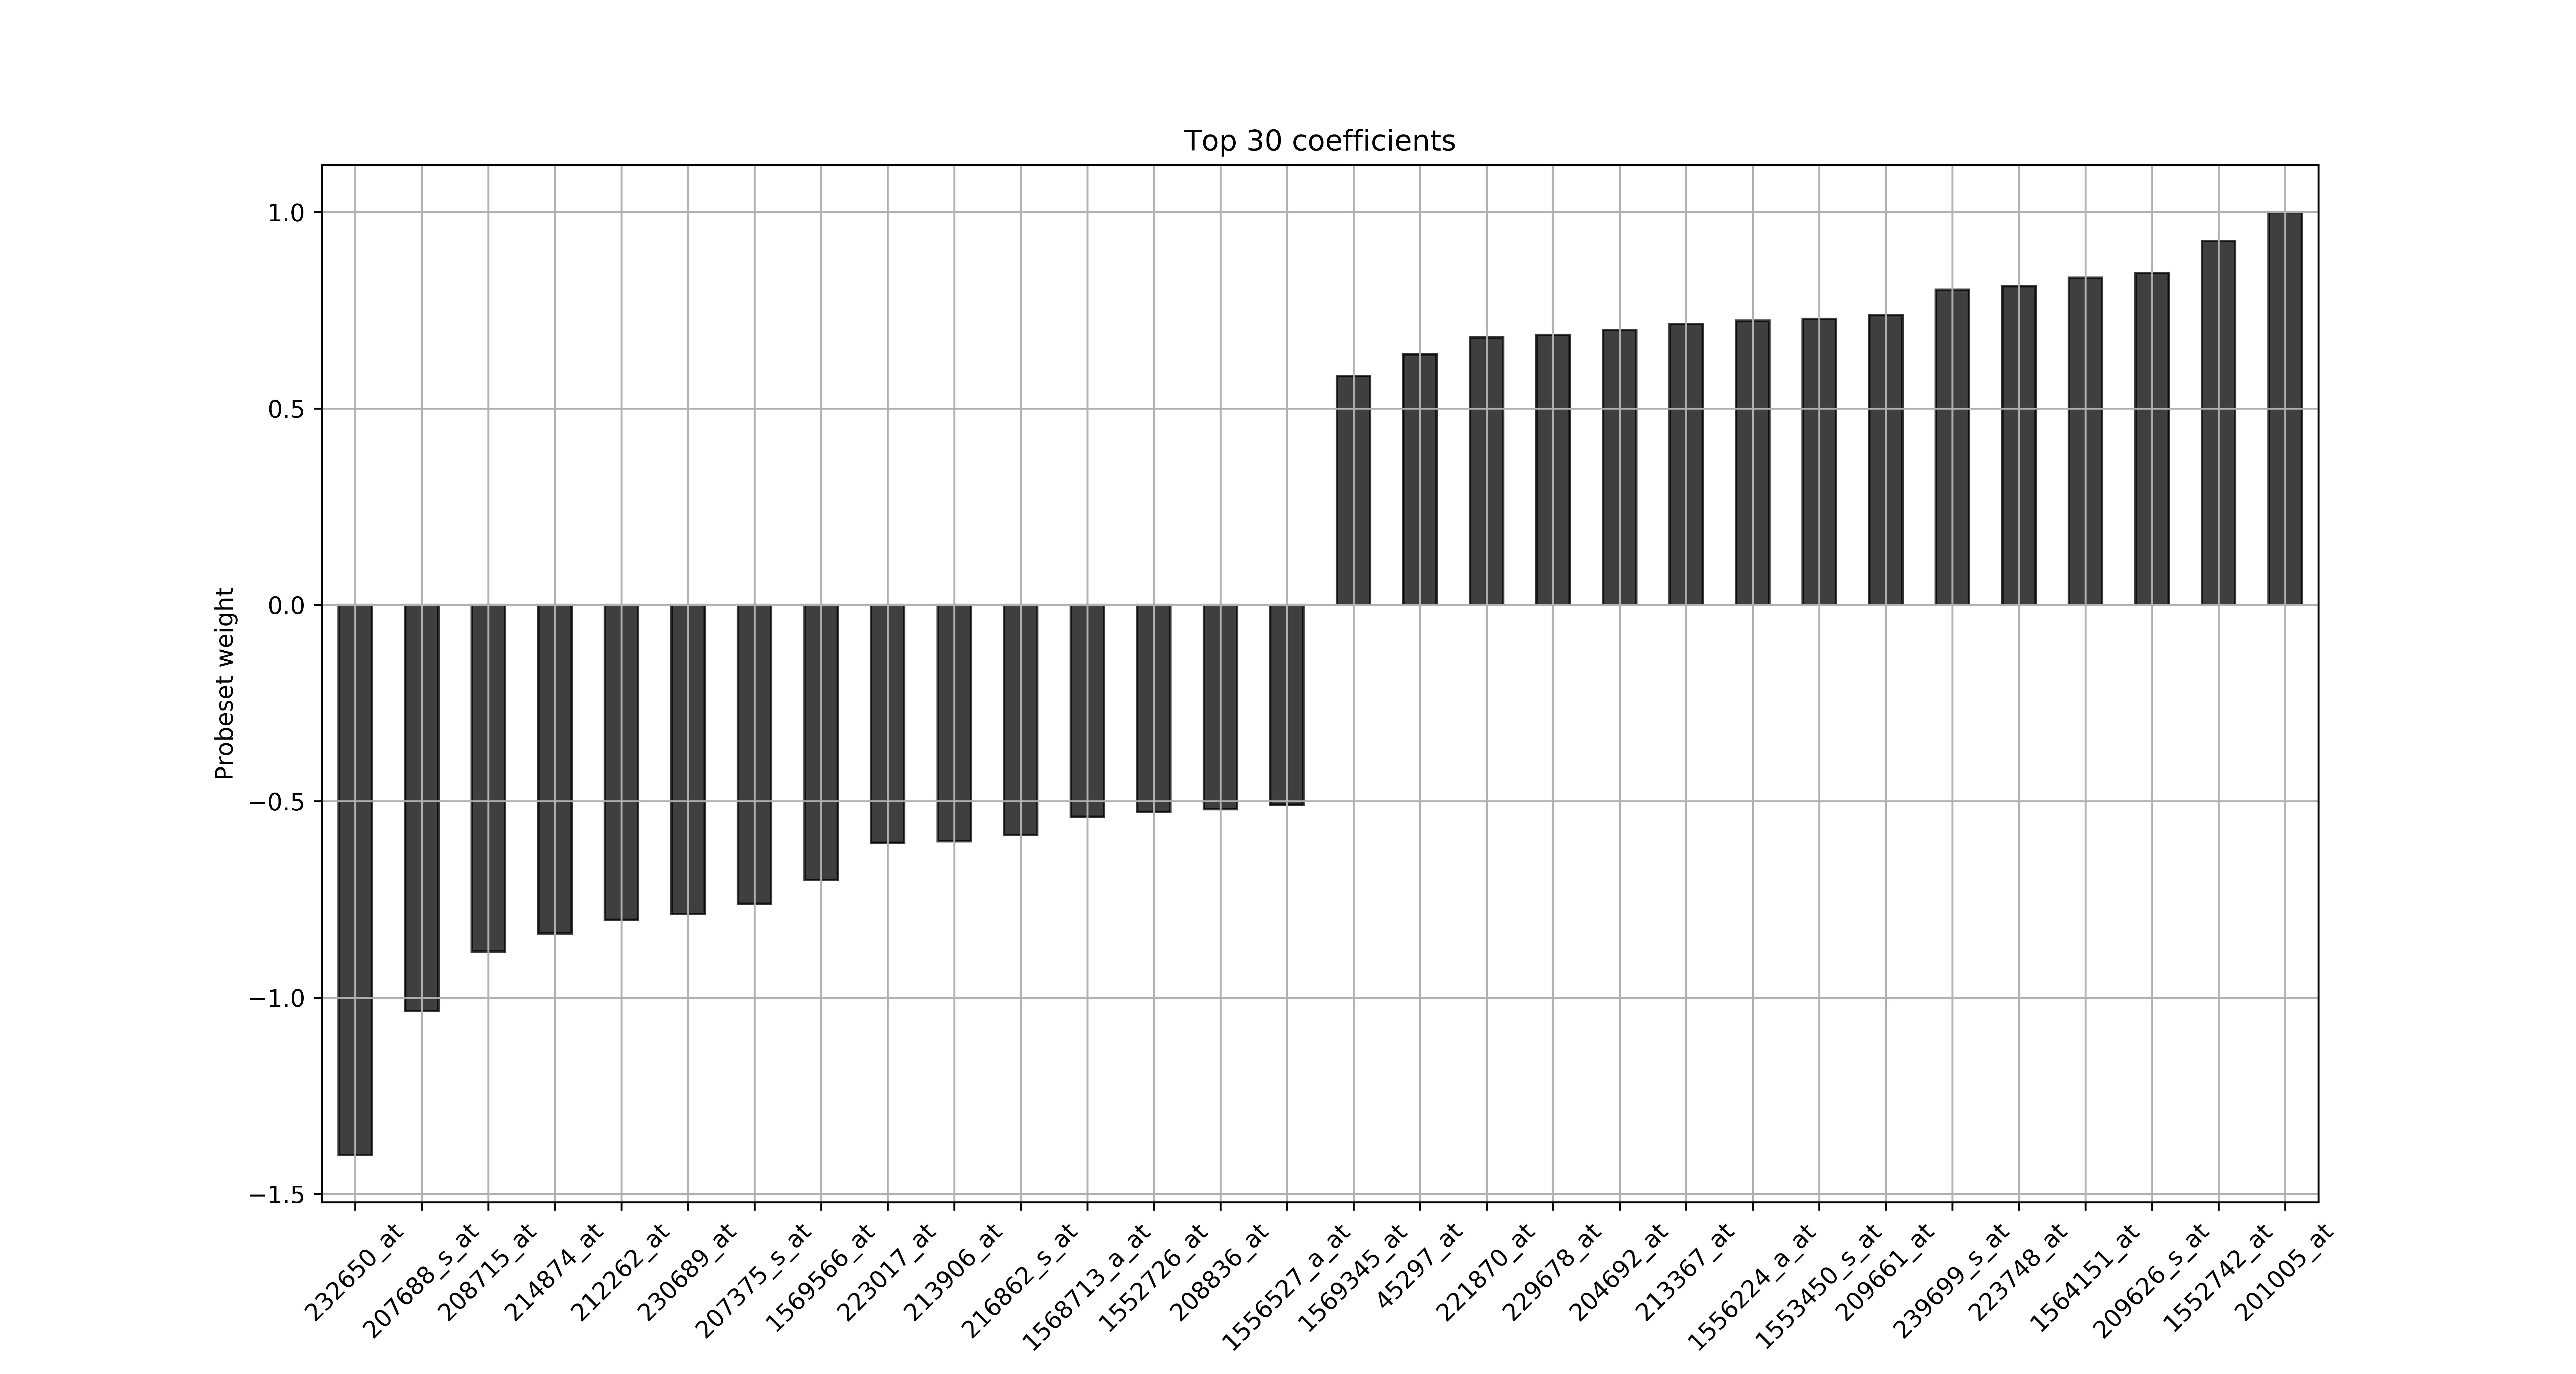
\includegraphics[width=12cm]{images/top30_weights_FDR005}
\caption{Top $30$ probesets in terms of median absolute weights for the lSVM and LR models}
\label{fig:coeffsFromModels}
\end{figure}
%
%
\section{Summarising}
%
For the cohort-bias removal we apply a genome-wise Location and scale (L/S) adjustment per cohort. This guarantees
similar bounds and means over the different cohorts. To remove the multiplicity of probesets per patients
we simply take the mean of the measurements per patient. Having obtained a normalised dataset we add $5\%$
of noise (with respect the maximum value) to increase the robustness of the final model. To further increase robustness, and improve 
interpretability we reduce the number of features by applying the FDR method with ANOVA for the distribution comparison, 
following the Benjamin-Hochberg procedure, using a maximum $p$-value of $0.05$. 
%
We have two data scenario's. Scenario $\mathcal{I}$ uses the data from adult patients with a known high/low intensity diagnosis (where 
medium intensity is considered equal to the low intensity diagnosis) to train a model to predict the diagnosis for the other non-labelled patients.
Scenario $\mathcal{II}$ uses the survival label of the patients as a proxy for the high/low intensity treatment. Now the training set from scenario
$\mathcal{I}$ is used as a validation set.
%
For the model creation we employ several \textit{tree-ensemble methods}: Random Forest (RF) by Breiman\cite{Breiman2001}, ExtraTrees (ET) by Geurts et al.\cite{Geurts2006} 
XGBoost (XGB) by Chen and Guestrin\cite{Chen2016} and (Light)GBM (LGBM) by Ke et al.\cite{Ke2017}. 
We use three types of linear methods, Linear Discrimination Analysis, Logistic Regression and linear SVM.
We use two nonlinear methods, both \textit{neural networks}, a Deep Neural Network (DNN) \cite{lecun2015deep} and a Convolutional Neural Network (CNN) \cite{Lecun98}.
Finally, we use two Bayesian methods, Naive Bayes and Gaussian Processes Classication (GPC).
%
Finally we combine them in a so-called stacked method, either by a majority vote of the classifications or by weighted averaging based on their prediction probabilities.
The benefit of combining these techniques is that we have the highest possible accuracy without compromising interpretability. \\ \\
%
Having obtained the models we can extract their relative importance from the tree-based models, and the weights from the linear models.
In our case we could reduce the more than $50.000$ expression values to about $200$ without losing accuracy. 
%
\section{Discussion}

\begin{itemize}
\item when choosing PCA, LDA, check for inflection point in eigenvalue magnitude to 'smartly' select the number of components
\item successively apply standard scaling and maxabs scaling to center cohort data?
\item improve bias removal method L/S by ignoring outliers during normalisation
\item instead of applying FDR once on the dataset, apply it several times on the same dataset with added noise to remove spurious contributors
\item we can combine the different models in one meta-model. This bagging of models increases the accuracy, removes method-specific biases and at the same time its helps reduce overfitting
\item the model generators that we applied, primarily used default parameter settings, we can likely improve the model quality by performing parameter optimisation
\end{itemize}

\section*{Appendix}
\subsection*{Model parameters}

\lstset{ 
  backgroundcolor=\color{white},   % choose the background color; you must add \usepackage{color} or \usepackage{xcolor}; should come as last argument
  basicstyle=\footnotesize,        % the size of the fonts that are used for the code
  breakatwhitespace=false,         % sets if automatic breaks should only happen at whitespace
  breaklines=true,                 % sets automatic line breaking
  captionpos=b,                    % sets the caption-position to bottom
  commentstyle=\color{mygreen},    % comment style
  deletekeywords={...},            % if you want to delete keywords from the given language
  escapeinside={\%*}{*)},          % if you want to add LaTeX within your code
  extendedchars=true,              % lets you use non-ASCII characters; for 8-bits encodings only, does not work with UTF-8
  frame=single,	                   % adds a frame around the code
  keepspaces=true,                 % keeps spaces in text, useful for keeping indentation of code (possibly needs columns=flexible)
  keywordstyle=\color{blue},       % keyword style
  language=Octave,                 % the language of the code
  morekeywords={*,...},            % if you want to add more keywords to the set
  numbers=left,                    % where to put the line-numbers; possible values are (none, left, right)
  numbersep=5pt,                   % how far the line-numbers are from the code
  numberstyle=\tiny\color{mygray}, % the style that is used for the line-numbers
  rulecolor=\color{black},         % if not set, the frame-color may be changed on line-breaks within not-black text (e.g. comments (green here))
  showspaces=false,                % show spaces everywhere adding particular underscores; it overrides 'showstringspaces'
  showstringspaces=false,          % underline spaces within strings only
  showtabs=false,                  % show tabs within strings adding particular underscores
  stepnumber=2,                    % the step between two line-numbers. If it's 1, each line will be numbered
  stringstyle=\color{mymauve},     % string literal style
  tabsize=2,	                   % sets default tabsize to 2 spaces
  title=\lstname                   % show the filename of files included with \lstinputlisting; also try caption instead of title
}
If any parameter is missing, please consult the documentation of the sklearn library (v. 0.19.1), 
the lightGBM library (v. 2.1.0), the XGboost library (v. 0.71) or Keras (v. 2.0.8).
\begin{verbatim}
            "GPC":{'optimizer': 'fmin_l_bfgs_b', 'n_restarts_optimizer': 0, 
                    'max_iter_predict': 100, 'warm_start': False, 
                    'copy_X_train': True, 'random_state': self.SEED, 
                    'multi_class': 'one_vs_rest', 'n_jobs': 1},
            "LDA":{'shrinkage': 'auto', 'solver': 'lsqr', 'priors': None},
            "LGBM": {'boosting_type':'gbdt' ,'learning_rate': 0.75, 
                    'max_depth': 4, 'num_leaves': 100, 'n_jobs': -1,
                    'n_estimators':100, 'random_state': self.SEED},  
            "XGB": {'seed': self.SEED, 'n_estimators': 100, 'max_depth': 3,
                    'learning_rate': 0.1, 'objective': 'reg:linear', 'nthread': -1},
            "ET": {'n_estimators': 50, 'max_depth': 15, 'n_jobs': -1, 
		  'min_samples_split': 10, 'min_samples_leaf': 5},
            "RF": {'n_estimators': 200, 'max_depth': 10, 'n_jobs': -1, 
		  'min_samples_split': 10, 'min_samples_leaf': 5},            
            "SVM":{'kernel': 'linear', 'gamma': 'auto', 'tol': 0.0005, 'C':  0.9, 
		  'probability' : True, 'max_iter': 3000},
            "LR": {'penalty':'l2', 'dual': False, 'tol':0.0001, 'C':0.9, 'max_iter': 100, 
		  'fit_intercept': True, 'intercept_scaling': 1},
\end{verbatim}

\bibliographystyle{plain}
\bibliography{methods}
\end{document}
